%%%% Paramétrage du TD %%%%
\def\xxactivite{TD 1 \ifprof -- Corrigé \else \fi} % \normalsize \vspace{-.4cm}
\def\xxauteur{\textsl{Xavier Pessoles}}


\def\xxnumchapitre{Chapitre 1 \vspace{.2cm}}
\def\xxchapitre{\hspace{.12cm} Correction des systèmes}


\def\xxcompetences{%
\vspace{-.3cm}
\textsl{%
\textbf{Savoirs et compétences :}\\
\vspace{-.4cm}
\begin{itemize}[label=\ding{112},font=\color{ocre}] 
%\item \textit{Res1.C4 : } Correction
 \item \textit{Res1.C4.SF1 : } Proposer la démarche de réglage d’un correcteur proportionnel
%proportionnel intégral 
%et à avance de phase
\item \textit{Con.C2 : } 	Correction d’un système asservi	
\item \textit{Con.C2.SF1 : } Choisir un type de correcteur adapté
\end{itemize}
}}

\def\xxauteur{\textsl{Xavier Pessoles}}

\def\xxtitreexo{Mobilité assistée à l'aide d'une canne robotisée \ifnormal $\star$ \else \fi \iftdifficile $\star\star\star$ \else \fi }
\def\xxsourceexo{\hspace{.2cm} \footnotesize{Concours CCP -- PSI 2018}}

\def\xxfigures{
%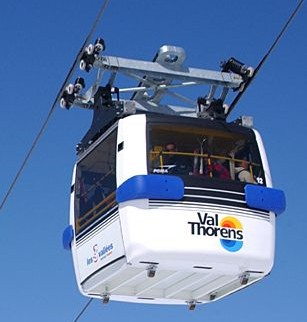
\includegraphics[width=.75\textwidth]{fig_00}
}%figues de la page de garde


\input{\repRel/Style/pagegarde_TD}
\setcounter{numques}{0}
\setlength{\columnseprule}{.1pt}

\pagestyle{fancy}
\thispagestyle{plain}

\vspace{5cm}

\def\columnseprulecolor{\color{ocre}}
\setlength{\columnseprule}{0.4pt} 

\setcounter{exo}{0}

\ifprof
%\begin{multicols}{2}
\else
\begin{multicols}{2}
\fi
%%%%%%%%%%%%%%%%%%%%%%%%%%%%%%%%%%%%%%%%%%%%%%%%%%





\subsection*{Présentation du prototype de canne robotisée étudié}
\ifprof
\else

L'objectif de cette canne est de prendre en charge une partie des efforts normaux supportés par une jambe handicapée.

Le prototype de canne robotisée envisagé conserve une forme longiligne, un point d'appui au sol ainsi qu'un encombrement et un poids réduits. La canne robotisée, dont la structure mécanique est présentée en \ref{fig:schema_general_canne}, se compose d'un axe linéaire motorisé et d'une roue motorisée située à son extrémité.


\begin{center}%[!ht]
%\centering
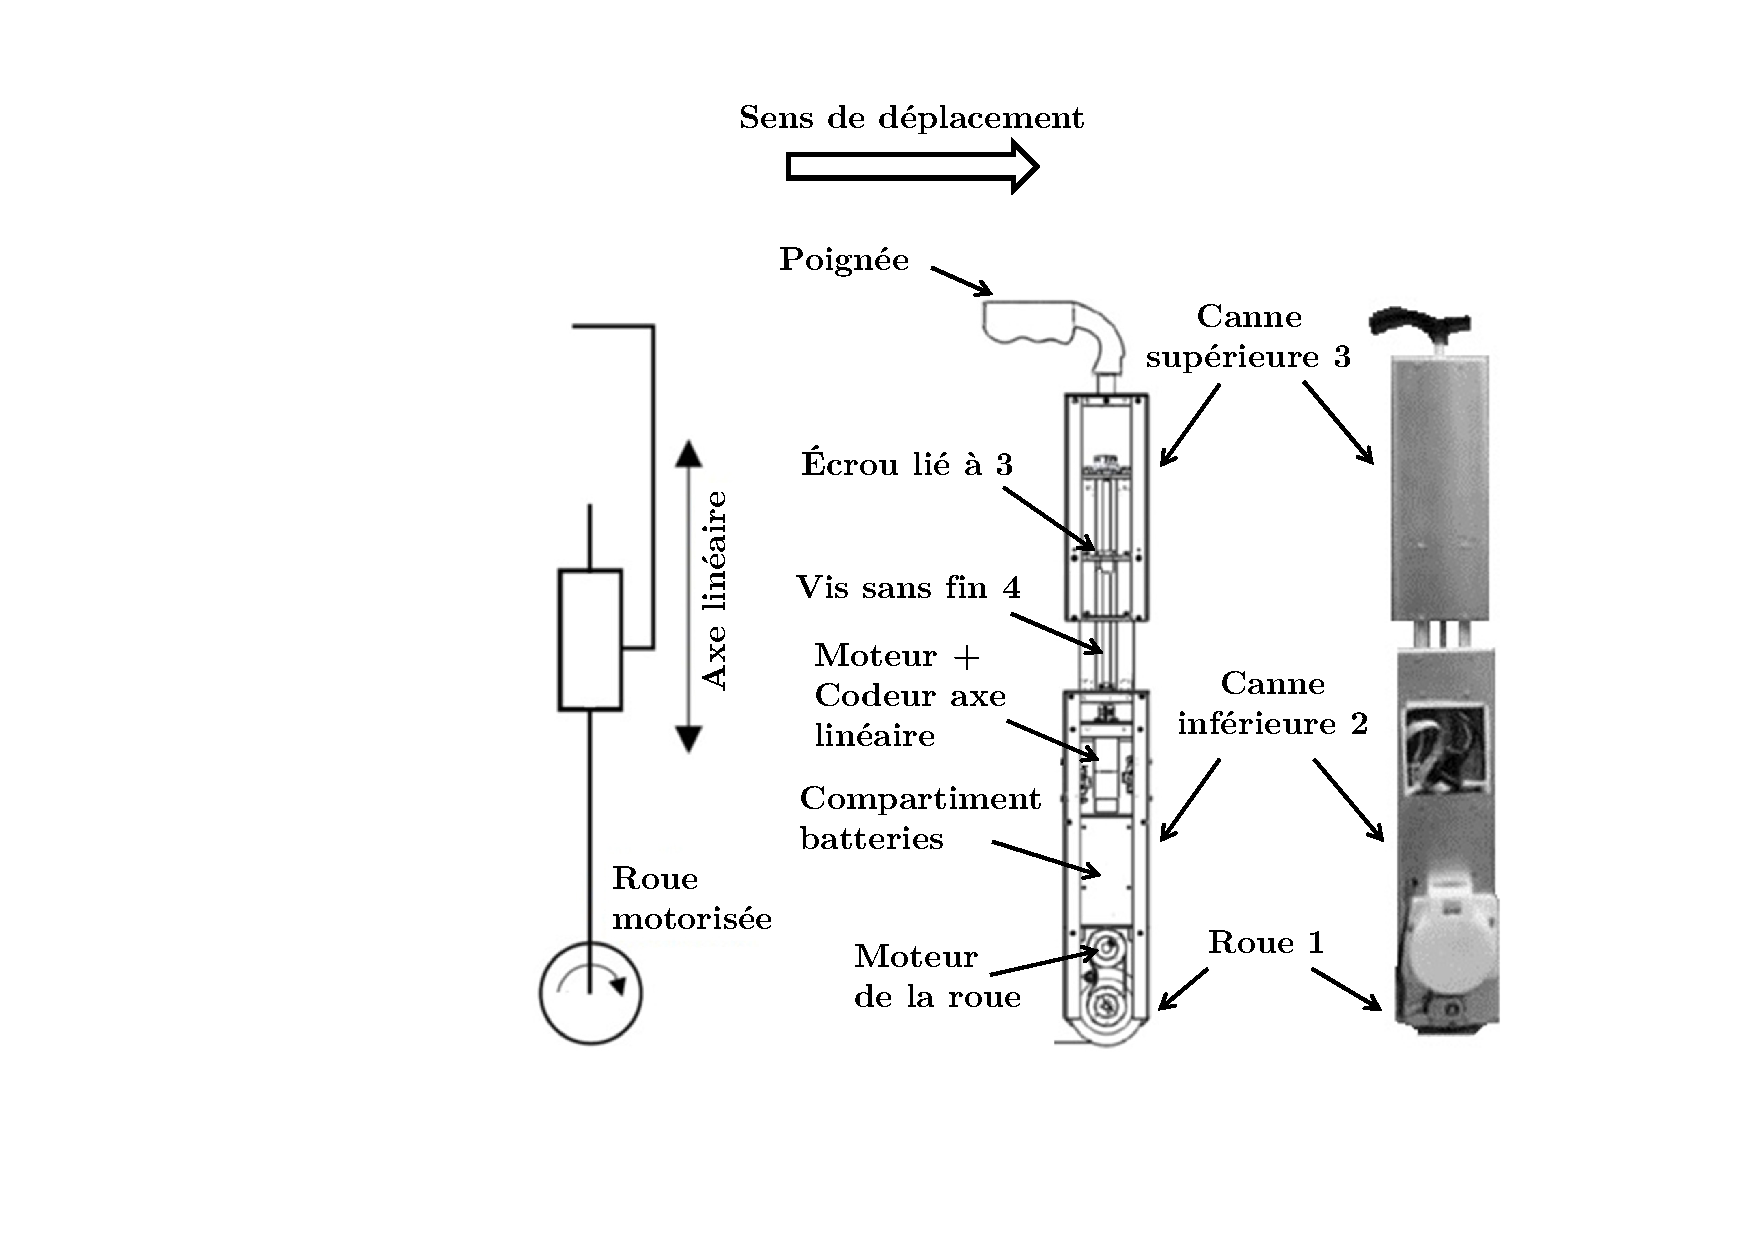
\includegraphics[width=\linewidth]{schema_general_canne2.pdf}
%\includegraphics[width=.6\linewidth]{schema_general_canne.jpg}
\captionof{figure}{{ Schéma cinématique et photographie du prototype de canne robotisée}}
\label{fig:schema_general_canne}
\end{center}


Les deux degrés de mobilité, rendus possibles par cette structure, permettent de suivre la marche d'un sujet et lui offre un point d'appui. L'avantage est d'éviter aux utilisateurs la manipulation de la canne (levée et positionnement) pendant la marche, la roue restant toujours en contact avec le sol.
%
%Le système de commande, détaillé par la suite, récupère les angles de rotation des deux centrales inertielles équipant respectivement la canne supérieure et le patient. La centrale inertielle du patient est placée sur la hanche de la jambe invalide et permet la synchronisation du mouvement de la canne avec celle-ci, comme nous le verrons par la suite.
%
%On donne dans le \ref{Annexe_diag_exigences} le diagramme partiel des exigences du prototype de canne robotisée.% 
%L'actionnement de l'axe linéaire de la canne est assuré par un moteur brushless Maxon ECMax 30 équipé d'un codeur incrémental. La roue 1, située à l'extrémité de la canne, est actionnée par un moteur brushless Maxon EC 60. Les caractéristiques des moteurs sont récapitulées dans le \ref{tab:donne_moteurs}.
%
%\begin{center}%[!ht]
%\centering
%\begin{footnotesize}
%\begin{tabular}{|p{5cm}|l|l|}
%  \cline{2-3}
%  \multicolumn{1}{c|}{} & \multicolumn{1}{|c|}{\textbf{Moteur axe linéaire}} & \multicolumn{1}{|c|}{\textbf{Moteur roue}}  \\ 
%  \multicolumn{1}{c|}{} & \multicolumn{1}{|c|}{brushless Maxon ECMax 30} & \multicolumn{1}{|c|}{brushless Maxon EC60} \\
%  \hline
%  Puissance maximale & $P_{\text{MAX}} = 60$ W & $P_{\text{\text{MAX}}} = 100$ W \\ 
%  
%  Vitesse nominale & $Nn = \num{6590}$ tr/min & $Nn = \num{3260}$ tr/min \\ 
%  
%  Couple nominal & $Cn = {0,0636}\ \si{N.m}$ & $Cn = \SI{0,279}{N.m}$ \\ 
%  
%  Tension nominale & $Un = 12$ V & $Un = 12$ V \\ 
%  
%  Courant nominal & $In = 4,72$ A & $In = 9,25$ A \\ 
%  
%  Courant maximal au démarrage & $I_{\text{\text{MAX}}}$ = 26,8 A &   {$I_{\text{\text{MAX}}}$ = 93,5 A} \\ 
%  
%%  \hspace*{1.5cm}  &  &  \\ 
%  
%  Constante de couple & $Kc = 14,2.10^{-3}$ \si{N.m/A} & $Kc = 30,5.10^{-3}$ \si{N.m/A} \\
%  
%  Constante de vitesse & $Ke = 14,2.10^{-3}$ V/s & $Ke = 30,5.10^{-3}$ V/s \\ 
%
%  Résistance aux bornes & $R = 0,447$ $\Omega$ & $R = 0,128$ $\Omega$ \\
%  
%  Inductance aux bornes & $L = 49 . 10^{-3}$ mH &  $L = 62 . 10^{-3}$ mH \\
%  
%  Moment d'inertie du rotor & $J_{\text{rotor}} = 21,9 . 10^{-7}$ \si{kg.m^2} & $J_{\text{rotor}} = 1,2 . 10^{-4}$ \si{kg.m^2} \\
%  \hline  
%\end{tabular} 
%\captionof{table}{{ Caractéristiques des moteurs brushless du prototype de canne}}
%\label{tab:donne_moteurs}
%\end{footnotesize}
%\end{center}
%
%\normalsize
%
%Le contrôle des moteurs est assuré par deux contrôleurs de vitesse ELMO. Ces variateurs reçoivent les consignes de vitesse du microcontrôleur MBED LPC1768. L'Arduino Due récupère les angles de deux centrales inertielles équipant la canne (par liaison série) et son utilisateur (par liaison Bluetooth).

\fi

%\subsection{Modélisation et analyse de la commande lors de la phase d'appui}
%\ifprof
%\else
%Cette étude permettra d'une part, de vérifier qu'il n'y aura pas glissement de la roue par rapport au sol lors de la phase d'appui et d'autre part, de comparer différents modèles de la structure asservie.
%\fi


\subsubsection*{Étude de l'exigence 3.1.6.2 \og Commande de l'axe linéaire\fg{}}
\ifprof
\else
 Le maintien d'une hauteur constante lors de la phase d'appui revient finalement à asservir en position le déplacement $x(t)$ de la canne supérieure 3 par rapport à la canne inférieure 2.

\begin{center}
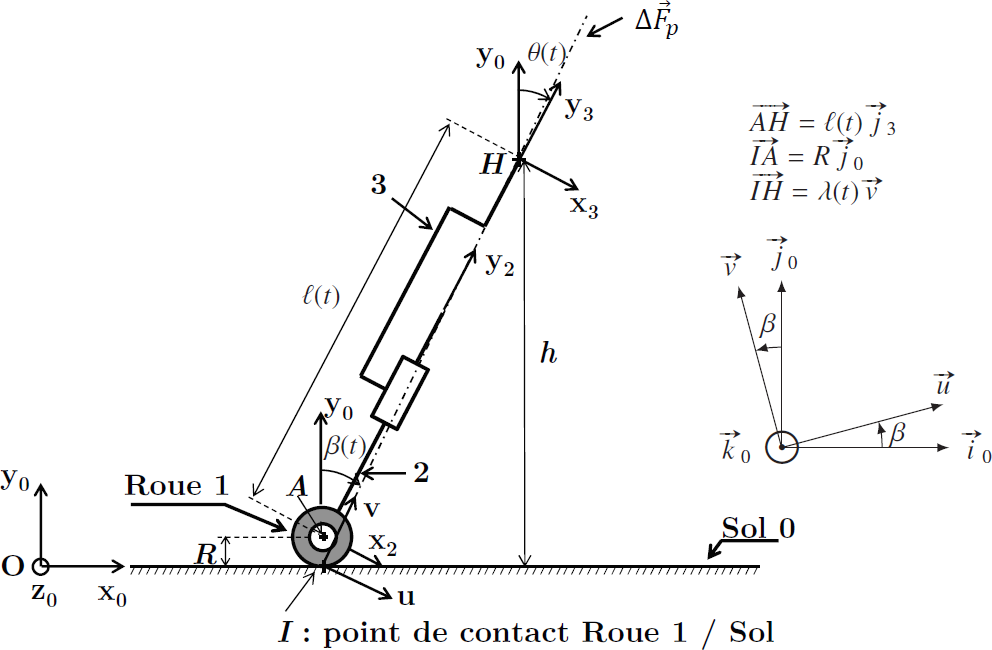
\includegraphics[width=.9\linewidth]{schema}
\end{center}
%Au cours de cette phase, l'angle de la hanche varie de \SI{+15}{\degree} à \SI{-10}{\degree}. Cette variation impose un déplacement relatif $x(t)$ quasi linéaire de l'ordre de quelques centimètres. Pour la suite, afin d'ajuster le réglage du correcteur réalisé par le contrôleur ELMO du moteur de l'axe linéaire, on se place dans le cas plus contraignant. Ce cas correspond à une consigne en échelon de 10 mm tout en prenant en compte l'action $F_p$ du patient en $H$, agissant ainsi comme une perturbation pour le déplacement $x(t)$.


Le modèle causal retenu pour l'étude du comportement de l'axe linéaire perturbé est représenté par le schéma-blocs ci-dessous. Dans ce modèle, on note :
\begin{itemize}
\item $X_c(p)$ la transformée de Laplace de la consigne de déplacement  $x_c(t)$ en mètre,
\item $X(p)$ la transformée de Laplace du déplacement $x(t)$ en mètre,
\item $F_p(p)$ la transformée de Laplace de   l'effort exercé par le patient sur la canne $F_p(t)$ en N,
\item $\Omega_m(p)$ la transformée de Laplace de la vitesse de rotation du moteur $\omega_m(t)$ en rad/s,
\item $C_m(p)$ la transformée de Laplace du couple moteur $C_m(t)$ en \si{N.m},
\item $C(p)$ la fonction de transfert du bloc correcteur.
\end{itemize}
\begin{center}
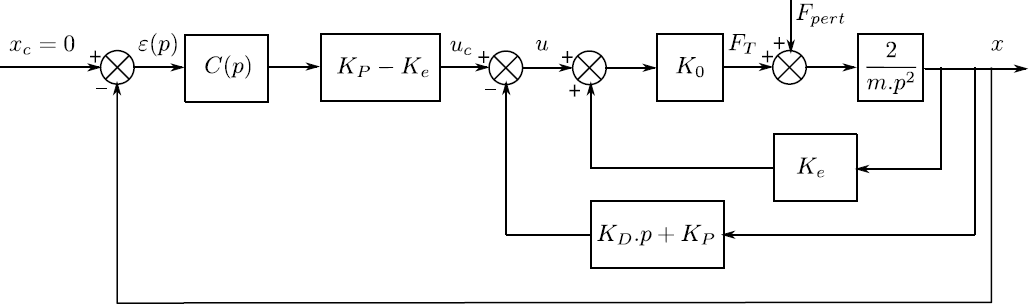
\includegraphics[width=\linewidth]{fig_02}
\end{center}
\fi
%
%\subsection*{Élaboration du modèle de connaissance de la partie dynamique de l'axe linéaire}
%\ifprof
%\else
%%\noindent Le modèle cinématique de l'axe linéaire retenu pour cette étude est donné en \ref{fig:schema_cine_Glissiere}.\\
%Les données et hypothèses de cette étude sont :
%\begin{itemize}
%\item le référentiel lié à la canne est supposé galiléen. Les effets d'inertie dus au mouvement de balancement sont donc négligés devant les autres grandeurs ;
%\item l'action du patient sur la canne supérieure 3 est considérée selon l'axe $(O_2,y_2)$, tel que \linebreak$\vect{F}_p(t) =  - F_p(t)\vect{j}_2$ ;
%\item l'ensemble des effets des frottements visqueux ramené au niveau de l'arbre moteur est \linebreak $f = 1,17.10^{-5}$ \si{N.m.s} ;
%\item la liaison glissière réalisée par deux douilles à billes est considérée sans frottement ;
%\item la vis 4 de moment d'inertie $J_{\text{vis}} = 1,53.10^{-6}$ \si{kg.m^2} est liée au rotor du moteur de moment d'inertie $J_{\text{rotor}} = 21,9.10^{-7}$ \si{kg.m^2} ;
%\item le pas de la vis sera noté $\text{pas}$ ;
%\item le couple qu'exerce le moteur sur la vis 4 est noté $C_m(t)$ ;
%\item la vitesse de rotation du moteur et de la vis sera notée $\omega_m(t)$ ;
%\item la vitesse de déplacement de 3 par rapport à 2 est notée $V_m(t)$ ;
%\item la masse de la canne supérieure est $M_3 = 1$ kg.
%%\item la masse de la canne inférieure est $M_2 = 4,7$ Kg.
%\end{itemize}
%
%%\begin{center}
%%
%%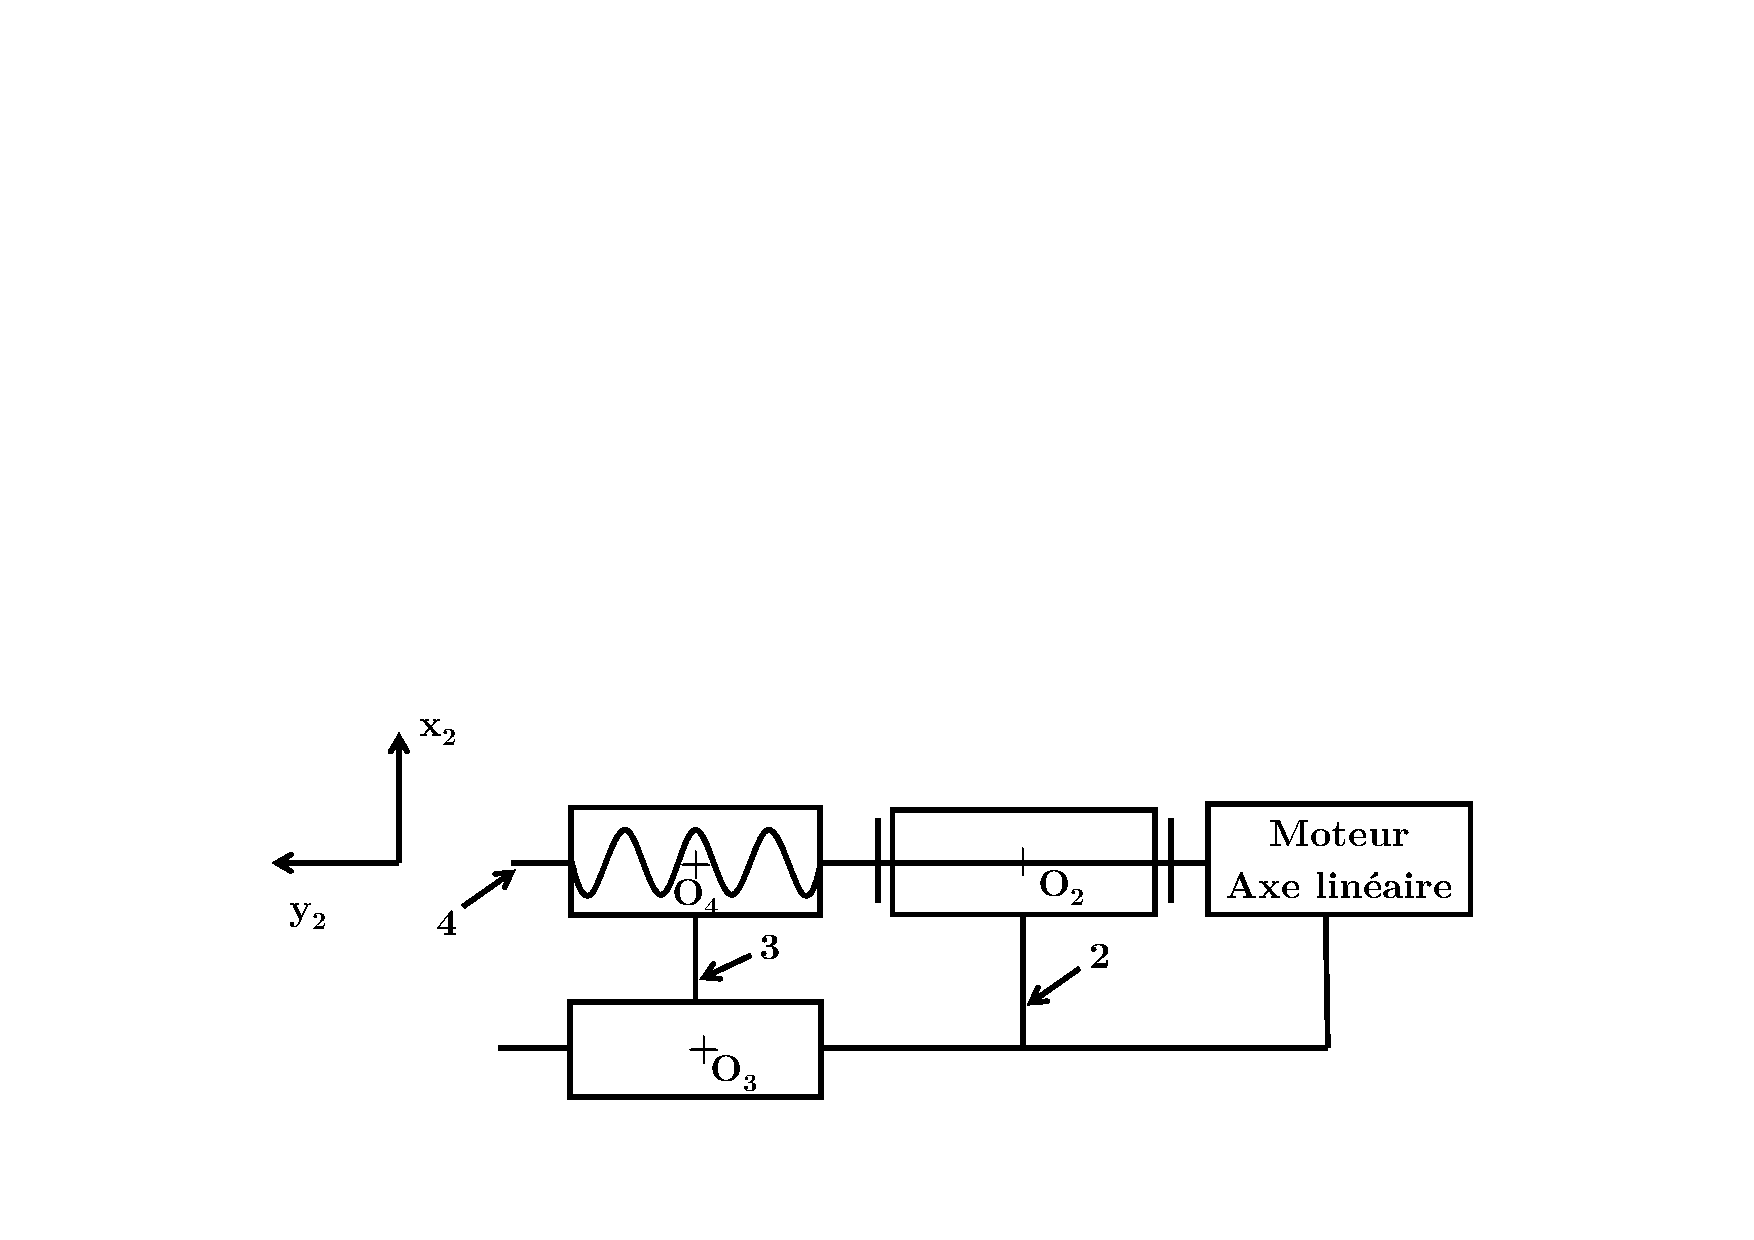
\includegraphics[width=0.65\linewidth]{schema_cine_Glissiere.pdf}
%%%\begin{minipage}[c]{.95\linewidth}
%%   \captionof{figure}{{ Modélisation cinématique de l'axe linéaire}
%%\label{fig:schema_cine_Glissiere}}
%%%\end{minipage}
%%\end{center}
%
%On isole l'ensemble $\mathcal{S} =\{3+4\}$.
%\fi
%
%L'équation du mouvement s'écrit $J_{eq} \dot{\omega}_m + f \omega_m = C_m - F_p  \frac{pas}{2\pi} $.
%
%\question{En supposant\label{Q:schema_bloc_1} les conditions initiales nulles, réaliser la transformée de Laplace de l'équation du mouvement précédente et compléter les blocs correspondants.}% du \DR{DR_schema_bloc}. }
%
%\ifprof
%\begin{corrige}
%En considérant nulle les conditions initiales, la transformée de Laplace de l'équation de mouvement est :\\
%$\left( J_{eq}.p + f \right).\Omega_m(p) = C_m(p) - \frac{pas}{2\pi}. F_p(p)$.\\
%On peut alors compléter les blocs du document réponse DR3.
%\end{corrige}
%
%
%\begin{center}
%\resizebox{.7\linewidth}{!}{
%\begin{tikzpicture}
%\sbEntree{B}
%\sbComp[5.5]{C2}{B}
%\sbBloc[1]{C}{$\dfrac{1}{R+L p}$}{C2}
%\sbBloc[1]{D}{$K_c$}{C}
%\sbComph[6]{C3}{D}
%\sbBloc[1]{E}{\textcolor{red}{$\dfrac{1}{f+J_{eq} p}$}}{C3}
%\sbSortie{S}{E}
%
%
%\sbRelier[$U_m(p)$]{B}{C2}
%\sbRelier{C2}{C}
%\sbRelier{C}{D}
%\sbRelier[$C_m(p)$]{D}{C3}
%\sbRelier{C3}{E}
%\sbRelier[ $\quad \quad \Omega_m(p)$]{E}{S}
%
%\sbDecaleNoeudy[4]{Ddroite}{H0}
%\sbBlocr[0]{H}{$K_e$}{H0}
%
%\sbRelieryx{E-S}{H}
%\sbRelierxy{H}{C2}
%
%\sbDecaleNoeudy[-4]{Ddroite}{J0}
%\sbBlocr[0]{J}{\textcolor{red}{$\dfrac{pas}{2\pi}$}}{J0}
%\sbDecaleNoeudx[-5]{J}{E2}
%\sbRelier[$F_p(p)$]{E2}{J}
%\sbRelierxy{J}{C3}
%
%\end{tikzpicture}}
%\end{center}
%
%\fi
%
%
%\subsection*{Modélisation de la chaîne d'énergie de l'axe linéaire}
%
%\ifprof
%\else
%On considère pour la suite que le moteur brushless adopte le même comportement que celui d'un moteur à courant continu. Les équations de comportement sont rappelées ci-après.
%
%$u_m(t)=e(t)+R.i_m(t)+L.\frac{\dd  i_m(t)}{\dd  t}$,
% $e(t) = K_e.\omega_m(t)$  et $C_m(t) = K_c.i_m(t)$.  
%
%
%On notera $U_m(p)$ respectivement $I_m(p)$, $C_m(p)$ et $E(p)$ les transformées de Laplace des variables $u_m(t)$ la tension moteur, respectivement $i_m(t)$, le courant moteur, $C_m(t)$, le couple moteur et $e(t)$, la force contre-électromotrice.
%
%Le dispositif vis/écrou permettant la transformation de l'angle de rotation de la vis (en radians) en déplacement de l'écrou (en mètre) est modélisé par le bloc de gain pur $K_{ve}$.
%Le comportement du codeur incrémental est modélisé par un gain pur $K_{\text{codeur}}$. On précise que la sortie de ce bloc est de type numérique (en incréments) et l'entrée est une position angulaire (en radians).
%\fi
%
%
%\question{Déterminer, à partir des données du diagramme de blocs internes, les expressions puis les valeurs numériques de $K_{ve}$ et $K_{\text{codeur}}$.}
%
%\ifprof
%\begin{corrige}
%D'après les données, $K_{ve} = \frac{pas}{2\pi} = \frac{3.10^{-3}}{2\pi} \simeq $ 4,77.10$^{-4}$ m/rad.\\
%Le codeur a une résolution de 500 impulsions par tour, donc $K_{\text{codeur}} = \frac{500}{2\pi} \simeq $ 79,6 imp/rad.
%\end{corrige}
%\fi
%
%\ifprof
%\else
%On place en amont du comparateur un bloc de gain pur $K_{\text{adapt}}$ de manière à convertir la consigne $X_c(p)$ en une grandeur en incréments directement comparable à la sortie $\theta_{\text{mes}}(p)$ du capteur. La valeur du gain pur $K_{\text{adapt}}$ est prise de manière à ce que l'écart $\varepsilon(p)$ soit nul lorsque $X_c(p) =  X(p)$.
%
%
%\fi
%
%\question{Donner l'expression, puis la valeur numérique du gain pur $K_{\text{adapt}}$ permettant de satisfaire cette condition.}
%\ifprof
%\begin{corrige}
%D'après le schéma-bloc, $\varepsilon(p) = K_{\text{adapt}}. X_c(p) - K_{\text{codeur}}.\frac{X(p)}{K_{ve}} $. Ainsi pour vérifier  $\varepsilon(p) = 0$ lorsque $X_c(p) =  X(p)$, il faut prendre :\\
%$K_{\text{adapt}} = \frac{K_{\text{codeur}}}{K_{ve}} $. L'application numérique donne $K_{\text{adapt}} = \frac{79,6}{4,77.10^{-4}} \simeq $ 166 700 imp/m.
%\end{corrige}
%\fi


\subsection*{Modèle comportemental}

\ifprof
\else
Afin de proposer une modélisation simplifiée de la chaîne d'énergie de l'axe linéaire, une simulation du modèle précédent en boucle ouverte, non perturbé, a été réalisée. Le document réponse présente la réponse fréquentielle du système en boucle ouverte à l'aide du diagramme de Bode (courbe de gain $G_{\text{BO}}(\omega)$ et courbe de phase $\varphi_{\text{BO}}(\omega)$). 


\fi



\question{À partir\label{Q_Bode} du diagramme de Bode, proposer un modèle de comportement du système en boucle ouverte. Soit $H_{BO\_1}(p)$ cette fonction de transfert, donner sa forme canonique factorisée. Soient $T_1$ et $T_2$, telles que $T_1 < T_2$, les constantes de temps introduites et $K_{\text{BO}}$ le gain de $H_{BO\_1}(p)$, préciser les valeurs numériques et unités de $T_1$, $T_2$ et $K_{\text{BO}}$. Vous laisserez apparaître les traits de construction nécessaires à l'identification du modèle sur le document réponse.}%}\DR{bode_BO_sans_corr}.}

\begin{center}
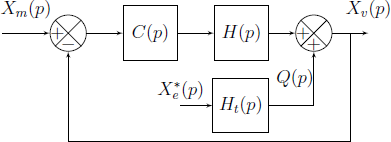
\includegraphics[width=\linewidth]{fig_03}
\end{center}


\ifprof
\begin{corrige}
L'allure des courbes de gain et de phase de la réponse fréquentielle du système en boucle ouverte montre clairement que le comportement est équivalent à celui d'un système du second ordre (avec coefficient d'amortissement $z>1$, car les courbes présentent deux cassures nettes en $\omega_{c1}=1/T_1$ et $\omega_{c2}=1/T_2$) associé à un intégrateur pur (pente de -20 dB/dec quand $\omega \rightarrow 0$ pour la courbe de gain et asymptote à -90\degre quand $\omega \rightarrow 0$ pour la courbe de phase). La forme canonique factorisée peut donc se mettre sous la forme : \\
$H_{BO\_1}(p) = K_{\text{BO}} . \frac{1}{p}. \frac{1}{1+T_1.p} . \frac{1}{1+T_2.p} $\\
On relève sur les courbes :\\
$\omega_{c1} \simeq 10^4$ rad/s, donc $T_1 = 10^{-4}$ s = 0,1 ms,\\
$\omega_{c2} \simeq 10^2$ rad/s, donc $T_2 = 10^{-2}$ s = 10 ms,\\
et en remarquant que pour $\omega = 10^0=1$ rad/s, $G_{\text{BO}}=20.log(K_{\text{BO}})= -30 dB$, on obtient $ K_{\text{BO}} = 10^{-30/20} \simeq $ 0,032 s$^{-1}$.
 \end{corrige}
\fi


\ifprof
\else

Lors d'une marche saine à allure rapide la cadence moyenne est de 113 pas par minute.
\fi

\question{Déterminer la fréquence moyenne en Hz de la marche saine à allure rapide.}

\ifprof
\begin{corrige}
Une cadence de 113 pas par minute correspond à une fréquence de marche de l'ordre de $\frac{113}{60} \simeq $ 1,88 Hz.
 \end{corrige}
\fi

\ifprof
\else
\vspace*{1em}
Pour la suite, on considérera que la fréquence maximale de déplacement de l'axe linéaire de  la canne (liée au mouvement de la marche) est fixée à $F_{\text{MAX}} = 4$ Hz. On propose alors en première approximation une modélisation du comportement du système en boucle ouverte par une fonction de transfert $H_{\text{BO}}(p)$ de la forme $H_{\text{BO}}(p) = K_{\text{BO}}/p$ avec $K_{\text{BO}} = 1/30$.
\fi

\question{Justifier, à l'aide de la réponse fréquentielle du système en boucle ouverte, la validité de cette modélisation approchée.}

\ifprof
\begin{corrige}
$F_{\text{MAX}} = 4$ Hz correspond à une sollicitation de pulsation $\omega_{\text{MAX}} = 4 \times 2 \pi \simeq $ 25 rad/s. \\
On constate que $\omega_{\text{MAX}}  <  \omega_{c2} = 100$ rad/s $<< \omega_{c1} = 10^{4}$ rad/s. \\
Pour $\omega < \omega_{\text{MAX}}$, le système se comporte donc comme un intégrateur pur de gain égal à $K_{\text{BO}}$. L'approximation de $H_{\text{BO}}(p)$ par $K_{\text{BO}}/p$ avec $K_{\text{BO}} = 1/30 \simeq 0,032$ est donc acceptable.
\end{corrige}
\fi

\ifprof
\else
%\vspace*{-1em}
\subsection*{Correction proportionnelle}

Pour la suite, on modélise le comportement du système en boucle ouverte par $H_{\text{BO}}(p) = K_{\text{BO}}/p$ avec $K_{\text{BO}} = 1/30$. On considère un correcteur à action proportionnelle tel que $C(p) = K_{\text{corr}} = 1$. \\
Le schéma-blocs du système non perturbé correspond alors à celui de la figure \ref{fig:schema_bloc_simplifie}.

%\begin{figure}[!ht]
%\centering
\begin{center}
\begin{tikzpicture}
\sbEntree{E1}
\sbComp{C1}{E1}
\sbBloc[2]{A}{$K_{\text{corr}}$}{C1}
\sbBloc[2]{B}{$\dfrac{K_{\text{BO}}}{p}$}{A}
\sbSortie[3]{S}{B}

\sbRelier[$X_c(p)$]{E1}{C1}
\sbRelier{C1}{A}
\sbRelier{A}{B}
\sbRelier[$X(p)$]{B}{S}

\sbRenvoi[3]{B-S}{C1}{}{}{}

\end{tikzpicture}%}
\captionof{figure}{{ Schéma-bloc  simplifié du système non perturbé avec $C(p) = K_{\text{corr}}$}
\label{fig:schema_bloc_simplifie}}
\end{center}

\fi


\question{Déterminer l'expression de $H_{\text{BF}}(p)= X(p)/X_c(p)$, la fonction de transfert en boucle fermée de la modélisation de la \ref{fig:schema_bloc_simplifie}. Déterminer les paramètres caractéristiques de $H_{\text{BF}}(p)$ et en déduire les performances de cette  modélisation pour $C(p) = K_{\text{corr}} = 1$. Conclure vis-à vis des performances d'asservissement de l'axe linéaire.}

\ifprof
\begin{corrige}
En appliquant la formule de Black, il vient $H_{\text{BF}}(p)= \frac{K_{\text{corr}}.K_{\text{BO}}/p}{1+K_{\text{corr}}.K_{\text{BO}}/p}$, avec $K_{\text{corr}} = 1$, on obtient :\\
$H_{\text{BF}}(p)= \frac{K_{\text{BO}}}{p+K_{\text{BO}}}$, soit sous forme canonique : $H_{\text{BF}}(p)= \frac{1}{1+\frac{1}{K_{\text{BO}}}.p}$.\\
La fonction de transfert est donc celle d'un système du 1er ordre, de gain unitaire $K_{\text{BF}}=1$ et de constante de temps $1/K_{\text{BO}} =$ 30 s.\\
Les performances de ce système sont donc :
\begin{itemize}
\item système stable car système du 1er ordre $ \Rightarrow $ cdcf vérifié,
\item système précis car de gain unitaire $ \Rightarrow $ cdcf vérifié,
\item système ne présente pas de dépassement car système du 1er ordre $ \Rightarrow $ cdcf vérifié,
\item tr$5\% = 3 \times 30 = 90$ s $ \Rightarrow $ cdcf non vérifié car le temps de réponse attendu est de 60 ms.
\end{itemize}
Le système avec $K_{\text{corr}} = 1$ est donc trop lent.
\end{corrige}
\fi

\ifprof
\else
\vspace*{1em}
On se propose de modifier la valeur de $K_{\text{corr}}$ de manière à vérifier l'exigence de rapidité de l'asservissement.
\fi

\question{Déterminer la valeur numérique à donner à $K_{\text{corr}}$ pour assurer le temps de réponse à 5\ \% lié à l'exigence de rapidité de l'asservissement de l'axe linéaire.}

\ifprof
\begin{corrige}
Il faut alors augmenter $K_{\text{corr}}$, tel que tr$5\% = 3 \times \frac{1}{K_{\text{corr}}.K_{\text{BO}}} \le 60$ ms. Donc \\
$K_{\text{corr}} \ge \frac{3}{60.10^{-3}.K_{\text{BO}}}$.
L'application numérique donne $K_{\text{corr}} \ge  1500$.
\end{corrige}
\fi


\ifprof
\else
La \ref{fig:reponse_Kcorr_1500}  donne l'évolution de la réponse temporelle $x(t)$ du système réel non perturbé à un échelon en déplacement de valeur finale $X_c = 10$ mm, pour une correction proportionnelle $K_{\text{corr}}$ = \num{1500}.


\begin{center}%[!ht]
%\centering


%\begin{minipage}[c]{.8\linewidth}
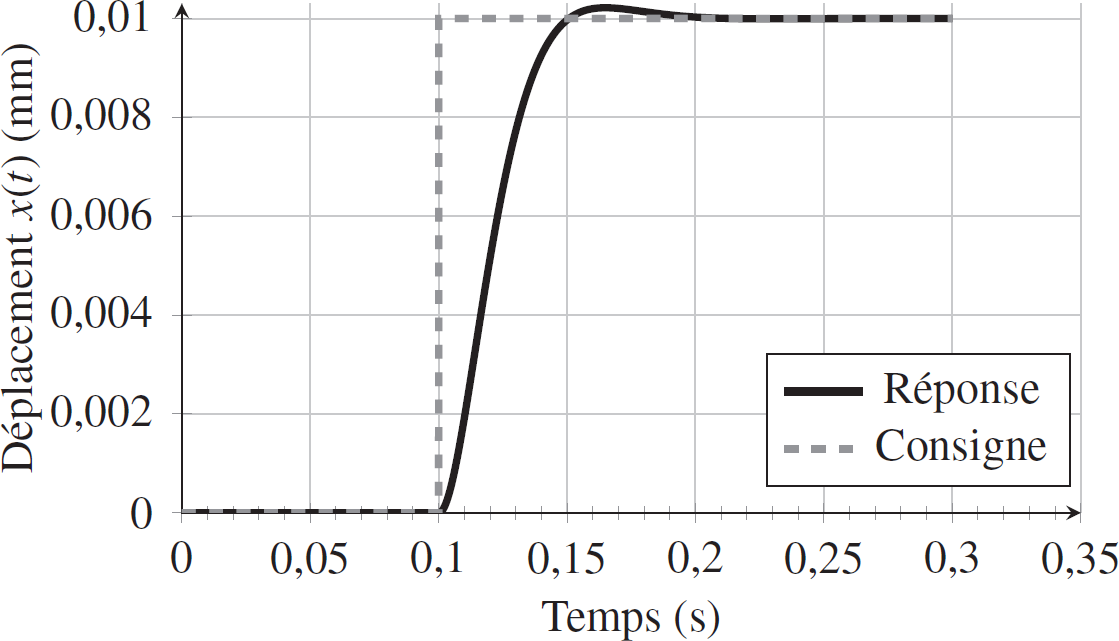
\includegraphics[width=.9\linewidth]{fig_11}
   \captionof{figure}{{ Évolution de la réponse temporelle $x(t)$ du système réel non perturbé à un échelon de valeur $X_c = 10$ mm, pour $K_{\text{corr}}$ = \num{1500}}\label{fig:reponse_Kcorr_1500}}
%\end{minipage}
\end{center}
\fi


\question{L'évolution de la réponse du système est-elle cohérente avec le comportement du modèle retenu ? Justifier. Quelle modification faudrait-il apporter au modèle approché pour retrouver cette forme de réponse temporelle ?}

\ifprof
\begin{corrige}
L'allure de la réponse ne correspond pas à celle d'un système du 1er ordre car un dépassement est observé. Avec $K_{\text{corr}} = 1500$, le système en boucle ouverte ne peut plus être modélisé par un intégrateur pur de gain $K_{\text{BO}}$, en effet cette valeur élevée de $K_{\text{corr}}$ fait monter la courbe de gain, le système a une bande passante plus élevée et l'action du terme $\frac{1}{1+T_2.p}$ ne peut plus être négligée. Le comportement du système doit donc être modélisé par celui d'un système du second ordre pour se rapprocher du comportement observé.
\end{corrige}
\fi

\ifprof
\else
Pour la suite, on modélise la fonction de transfert en boucle ouverte du système par \linebreak $H_{\text{BO}}(p) = \frac{1}{p}.\frac{K_{\text{BO}}}{1+\tau_{\text{BO}}p}$ avec $K_{\text{BO}} = 1/30$ (unité en \si{s^{-1}}) et $\tau_{\text{BO}} = 9$ ms.
\fi

\question{Quelle valeur maximale de $K_{\text{corr}}$, notée $K_{\text{corr}}^{\text{\text{MAX}}}$, permet de vérifier les critères de précision et de dépassement de l'asservissement de l'axe linéaire ?}

\ifprof
\begin{corrige}
Le critère de précision est satisfait du fait de la présence du terme intégrateur en $\frac{1}{p}$ dans la fonction de transfert en boucle ouverte du système.\\
Pour assurer un 1er dépassement $D1\% \leq 5 \%$, il faut que le système du second ordre ait un coefficient d'amortissement $z$, tel que $z \ge 0,7$. On détermine l'expression de $H_{\text{BF}}(p)$, la fonction de transfert en boucle fermée, afin d'identifier $z$.\\
D'après la formule de Black, $H_{\text{BF}}(p) = \frac{K_{\text{corr}}.H_{\text{BO}}(p)}{1+K_{\text{corr}}.H_{\text{BO}}(p)} = \frac{K_{\text{corr}}.K_{\text{BO}}}{K_{\text{corr}}.K_{\text{BO}} + p.\left( 1+ \tau_{\text{BO}}.p \right)}$.

La forme canonique de $H_{\text{BF}}(p)$ est donc :
$H_{\text{BF}}(p) = \frac{1}{1+\frac{1}{K_{\text{corr}}.K_{\text{BO}}}.p+ \frac{\tau_{\text{BO}}}{K_{\text{corr}}.K_{\text{BO}}}.p^2} $

Par identification,
$\omega_0 = \sqrt{\frac{K_{\text{corr}}.K_{\text{BO}}}{\tau_{\text{BO}}}} $ et $z=\frac{1}{2}.\omega_0.\frac{1}{K_{\text{corr}}.K_{\text{BO}}}$,
donc, $z = \frac{1}{2}.\frac{1}{\sqrt{\tau_{\text{BO}}.K_{\text{corr}}.K_{\text{BO}}}}$.
La condition $z \ge 0,7$ implique donc $K_{\text{corr}} \leq \frac{1}{(2 \times 0,7)^2.\tau_{\text{BO}}.K_{\text{BO}}}$.
L'application numérique donne $K_{\text{corr}} \leq 1700$. On prend donc $K_{\text{corr}}^{\text{\text{MAX}}} = 1700$.
\end{corrige}
\fi



\question{Déterminer la valeur du temps de réponse à $5\ \%$, $t_{r5\%}$ de ce modèle pour $K_{\text{corr}} = K_{\text{corr}}^{\text{\text{MAX}}}$ à partir de l'abaque du temps de réponse réduit donné ci-dessous.}
\ifprof
\else
\begin{center}
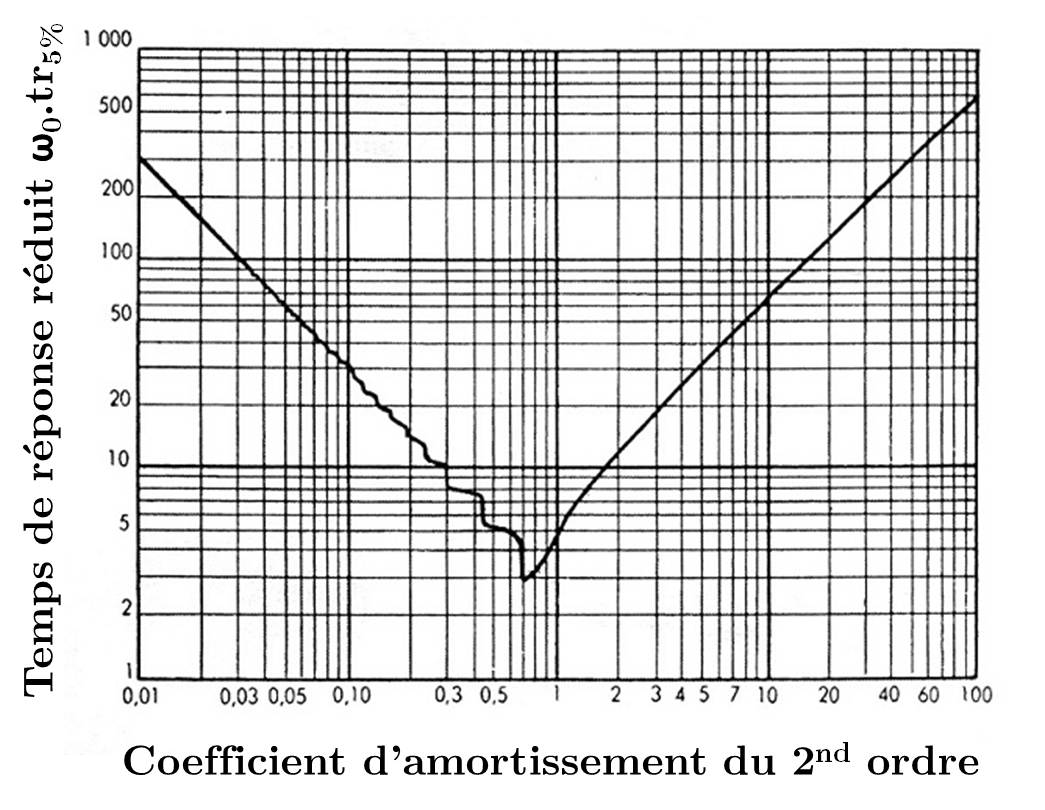
\includegraphics[width=.9\linewidth]{Abaque_tr_reduit.jpg}
\end{center}
\fi

\ifprof
\begin{corrige}
D'après l'abaque du temps de réponse réduit donné en \ref{Annexe_Abaque_tr_reduit}, pour $z = 0,7$ on relève $tr_{5\%}.\omega_0 \simeq 3$. Or $\omega_0 = \sqrt{\frac{K_{\text{corr}}^{\text{\text{MAX}}}.K_{\text{\text{BO}}}}{\tau_{\text{\text{BO}}}}} $, donc $tr_{5\%} = 3.\sqrt{\frac{\tau_{\text{\text{BO}}}}{K_{\text{corr}}^{\text{\text{MAX}}}.K_{\text{BO}}}}$. \\
L'application numérique donne : $tr_{5\%} \simeq $ 38 ms $<$ 60 ms $ \Rightarrow $ cdcf vérifié !
\end{corrige}
\fi


\ifprof
\else
%\newpage
La figure  \ref{fig:reponse_kcorr_kcorrmax} donne les évolutions des réponses temporelles $x(t)$ du système réel avec prise en compte de la perturbation ($F_p$ constante et égale à 175 N) à un échelon en déplacement de valeur finale $X_c = 10$ mm, pour une correction proportionnelle $K_{\text{corr}} = \num{1500}$ et pour $K = K_{\text{corr}}^{\text{\text{MAX}}}$.

\begin{center}%[!ht]

\iflivret
\begin{center}
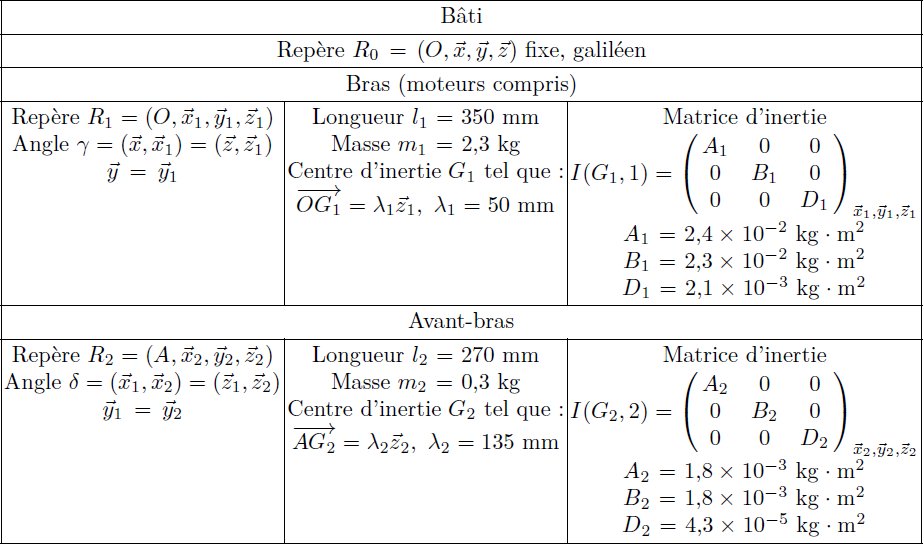
\includegraphics[width=\linewidth]{fig_06}
\end{center}
\else
%\centering
%\includegraphics[width=0.6\linewidth]{reponse_kcorr_kcorrmax.pdf}
\begin{tikzpicture}
\begin{axis}[
grid=major,tick label style={/pgf/number format/fixed},scaled ticks=false,/pgf/number format/1000 sep = {\,},/pgf/number format/use comma,
ytick={0,0.002,0.004,.006,.008,.01,0.012},
yticklabels={0,\num{0.002},\num{0.004},\num{.006},\num{.008},\num{.01},\num{0.012}},
%minor y tick num=3,
minor x tick num=4,
xlabel = {Temps (s)},
ylabel = {Déplacement $x(t)$ (mm)},
legend entries={$K_{\text{corr}}=K_{\text{corr}}^{\text{\text{MAX}}}$,$K_{\text{corr}}=\num{1500}$,Consigne},
legend style={at={(0.55,0.05)},anchor=south west},
%legend columns=3,
axis lines=left,
xmin=0,xmax=.35,
ymin=0,ymax=0.0103,
height=5.5cm,
width=8.5cm,
font=\footnotesize,
]
\addplot [ultra thick] table[x index=0,y index =3,col sep=semicolon]{images/reponse_pert.csv};
\addplot [gray,ultra thick] table[x index=0,y index =1,col sep=semicolon]{images/reponse_pert.csv};
\addplot [gray,dashed, ultra thick] table[x index=0,y index =2,col sep=semicolon]{images/reponse_pert.csv};
\end{axis}
\end{tikzpicture}
\fi

%\begin{minipage}[c]{.8\linewidth}
   \captionof{figure}{{ Réponses temporelles $x(t)$ du système réel perturbé à un échelon en déplacement de valeur finale $X_c = 10$ mm, pour une correction proportionnelle $K_{\text{corr}} = \num{1500}$ et pour $K = K_{\text{corr}}^{\text{\text{MAX}}}$}
\label{fig:reponse_kcorr_kcorrmax}
}
%\end{minipage}
\end{center}
\fi

\question{Conclure sur les capacités de la correction à action proportionnelle pure vis-à-vis des performances à atteindre.}
\ifprof
\begin{corrige}
Les performances de stabilité, rapidité et de 1er dépassement sont vérifiées. Cependant, le système avec correction proportionnelle n'arrive pas à atténuer suffisamment la perturbation (l'erreur est de l'ordre de 15 à 20$\%$ bien supérieure au 5$\%$ du cahier des charges). Un autre type de correction doit donc être envisagé pour satisfaire l'ensemble des critères.\end{corrige}
\fi


\ifprof
\else
%\vspace{-1em}
\subsection*{Correction avec action proportionnelle et intégrale généralisée -- correcteur PI généralisé}

%Les résultats des corrections précédentes montrent qu'il est nécessaire d'introduire une action dérivée pour augmenter les marges de Gain et de Phase du système en boucle ouverte.

Le correcteur finalement retenu est un correcteur avec action proportionnelle et intégrale généralisée. La fonction de transfert $C(p)$ prend alors la forme suivante :

{\centering
$C(p)= K_{\text{corr}} . \frac{1+T_d p}{p}$  avec $K_{\text{corr}} >> 1$ et $T_d < 1$ s.
\par}
On donne dans le document réponse le diagramme de Bode (courbe de Gain et de Phase) du système en boucle ouverte avec correcteur PI Généralisé pour $K_{\text{corr}} = \num{1000}$ et $T_d = 0,2$ s. 
\fi

\question{Représenter sur le document réponse les marges de Gain $M_G$ et de Phase $M_{\phi}$ du système corrigé.\label{Q:Bode_corrige}}

\ifprof
\begin{corrige}
D'après la figure ci-dessous, on relève une marge de Gain $M_G \simeq$ 60 dB et une marge de Phase $M_{\varphi} \simeq$ 50\degre. Avec ces valeurs le cahier des charges ($M_G =$ 45 dB et $M_{\varphi} =$ 35\degre) est vérifié.
 
 
%\begin{figure}[!ht]
%   \begin{minipage}[c]{.95\linewidth}
%      \centering
\begin{center}
      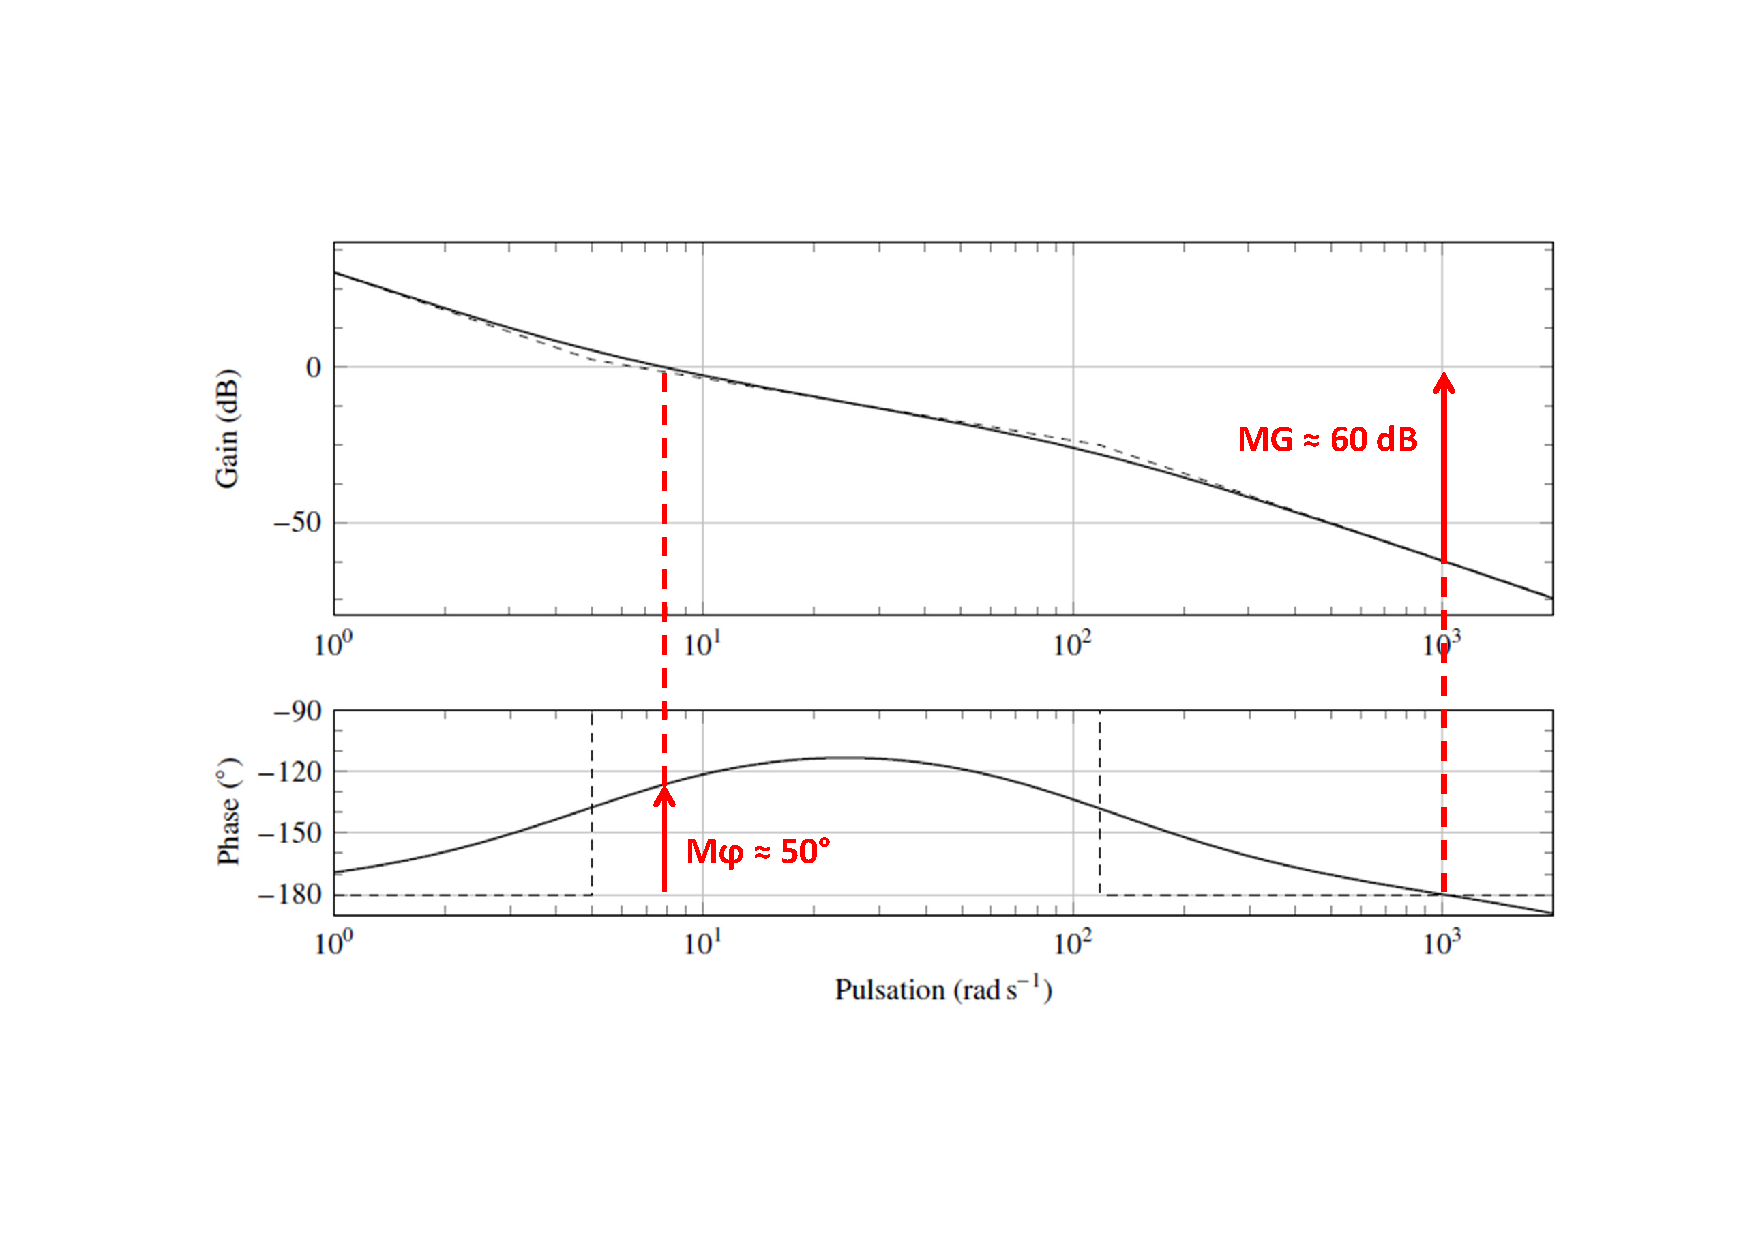
\includegraphics[width=1\linewidth]{Bode_correction_int_pure_marge}
\end{center}
%   \end{minipage}
%\end{figure}
\end{corrige}
\fi

\ifprof
\else
Avec cette correction, le système est précis mais les valeurs des marges de gain et de phase sont telles que le système n'est pas assez rapide. Il est donc nécessaire d'augmenter la valeur de $K_{\text{corr}}$, tout en conservant $T_d = 0,2$ s, de manière à augmenter la bande passante du système et ainsi se rapprocher des valeurs limites de marge de Gain et de Phase autorisées.
\fi

\question{En déduire la valeur maximale à donner au gain $K_{\text{corr}}$, en conservant $T_d = 0,2$ s, afin de respecter les performances en stabilité de l'asservissement de l'axe linéaire tout en augmentant au maximum la bande passante du système. }


\begin{center}
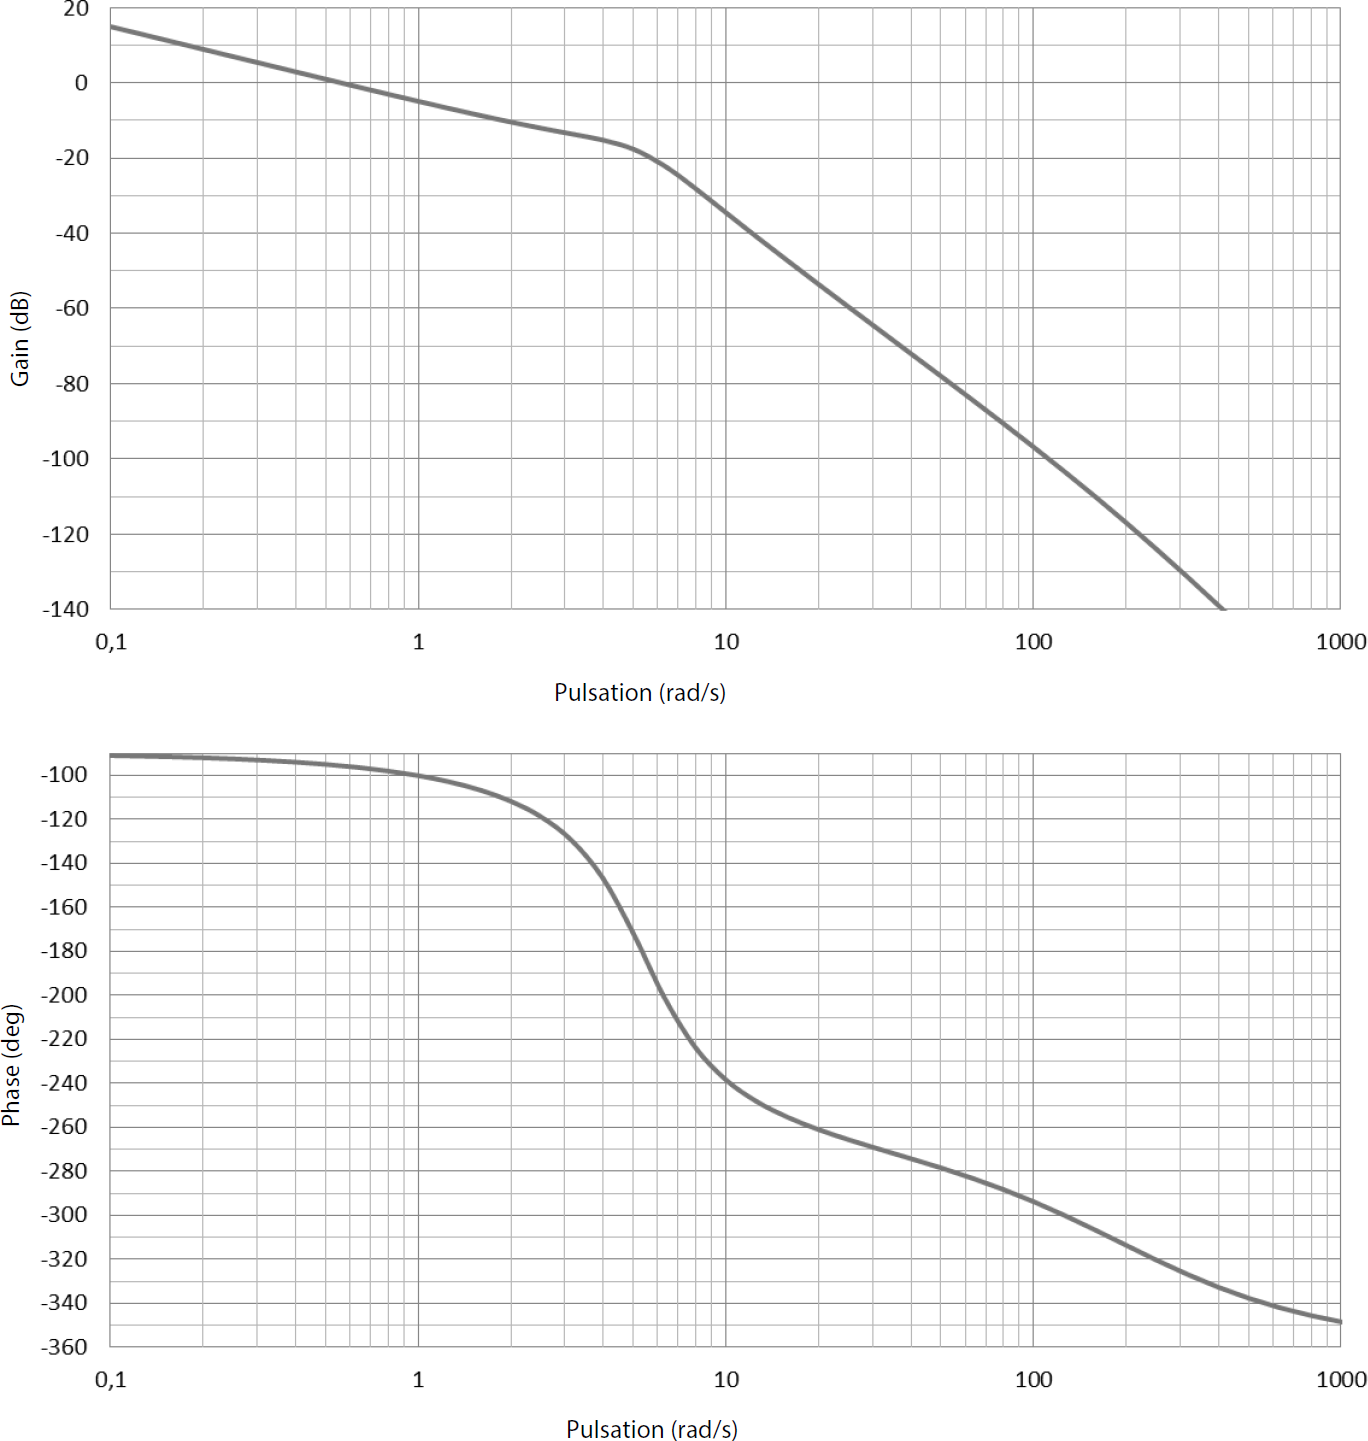
\includegraphics[width=\linewidth]{fig_04}
\end{center}

\ifprof
\begin{corrige}
La modification de la valeur du gain $K_{\text{corr}}$ n'affecte que la courbe de gain. L'augmentation de $K_{\text{corr}}$ va faire remonter la courbe de gain du système en boucle ouverte. Graphiquement, on observe que c'est le critère sur la marge de Gain qui limite la remonté de la courbe de gain (voir figure ci-dessous). La courbe de gain peut donc être remontée de +15 dB, on relève alors une marge de Gain $M_G \simeq$ 45 dB et une marge de Phase $M_{\phi} \simeq$ 65\degre. \\
Initialement on avait $K_{\text{corr}}^{init} = 1000$, pour remonter la courbe de gain de +15 dB, il faudra prendre $K_{\text{corr}}^{new}$ tel que : \\
$20 \times log(K_{\text{corr}}^{new}) = 20 \times log(K_{\text{corr}}^{init}) + 15$\\
$\Leftrightarrow K_{\text{corr}}^{new} = K_{\text{corr}}^{init} \times 10^{15/20}$\\
L'application numérique donne $K_{\text{corr}}^{new} \simeq$ 5620. 
 
 
\begin{center}
       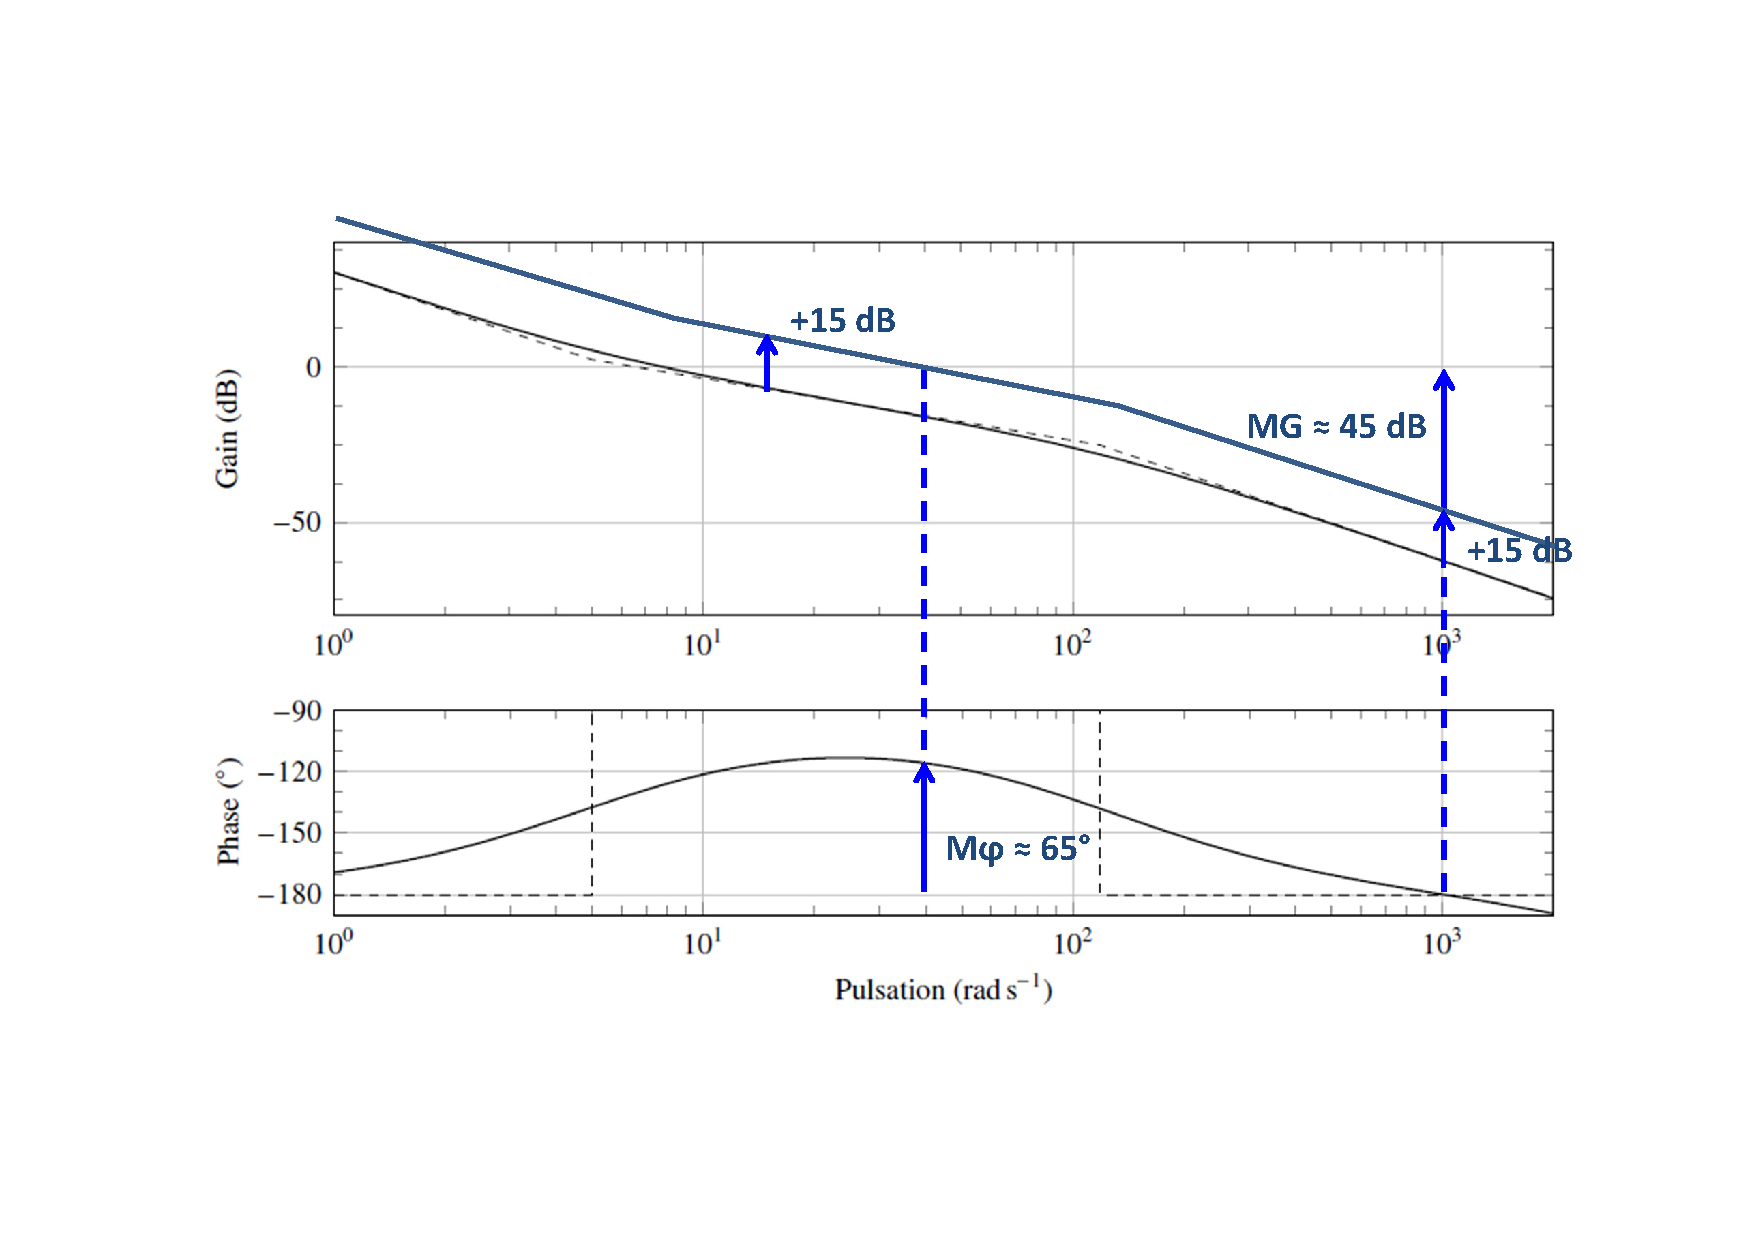
\includegraphics[width=.8\linewidth]{Bode_correction_int_pure_lim_marge}

 \end{center} 

\end{corrige}
\fi

\ifprof
\else
\vspace{1em}
%La \ref{fig:reponse_perturbe_corr_PI_gen}\textbf{(a)} donne la réponse temporelle à un échelon de consigne $X_c = 10$ mm du système simulé, perturbé et corrigé. La \ref{fig:reponse_perturbe_corr_PI_gen}\textbf{(b)} donne l'évolution de l'intensité simulée (en Ampères) circulant au sein du moteur lors de cette réponse.   
Les figures \ref{fig:reponse_perturbe_corr_PI_gen} donnent la réponse temporelle à un échelon de consigne $X_c = 10$ mm du système simulé, perturbé et corrigé du déplacement $x(t)$ (en mm)  ainsi que l'évolution de l'intensité simulée (en Ampères) circulant au sein du moteur.

\begin{center}
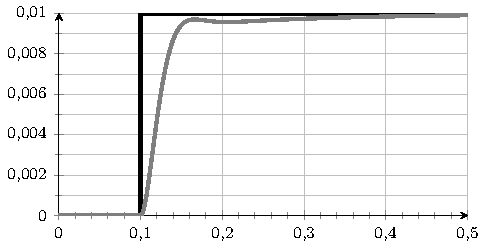
\includegraphics{reponse_temp_pert_a}
\textit{Déplacement (mm) en fonction du temps~(s)}

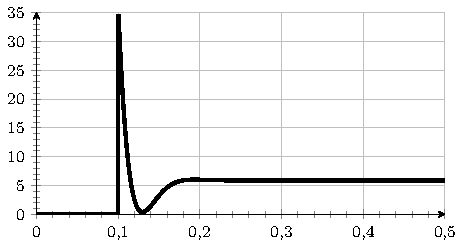
\includegraphics{reponse_temp_pert_b}
\textit{Intensité simulée (A) en fonction du temps~(s)}

 \captionof{figure}{Réponses temporelles à un échelon d'amplitude $X_c = 10$ mm du système simulé, perturbé et corrigé \label{fig:reponse_perturbe_corr_PI_gen}}
\end{center}

\fi


\question{Conclure sur les performances du système perturbé vis-à-vis des exigences de l'asservissement de l'axe linéaire. Commenter l'évolution de l'intensité simulée avec les caractéristiques de la carte de commande du moteur.}


\ifprof
\begin{corrige}
Avec cette correction la réponse temporelle respecte l'ensemble des critères du cahier des charges :\\
- le système est stable et $M_G \simeq$ 45 dB et $M_{\phi} \simeq$ 65\degre $ \Rightarrow $ cdcf vérifié,\\
- le système est précis $ \Rightarrow $ cdcf vérifié,\\
- système ne présente pas de dépassement $ \Rightarrow $ cdcf vérifié,\\
- tr$5\% \simeq$ 50 ms $ \Rightarrow $ cdcf vérifié (< 60 ms).\\
Par contre, on relève un courant $I_{mot}^{\text{\text{MAX}}} \simeq$ 35 A. Or la carte ELMO ne supporte qu'un courant maximal de 20 A. Le contrôleur ELMO ne permet donc pas de réaliser cette commande. 


\begin{center}
      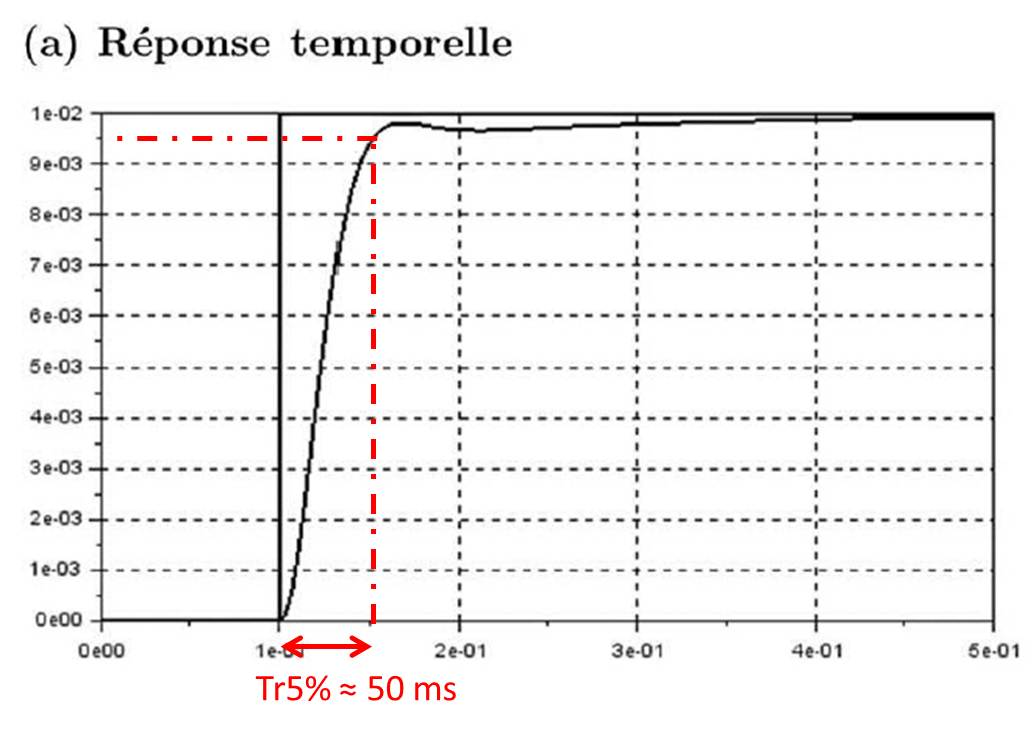
\includegraphics[width=0.7\linewidth]{reponse_perturbe_corr_PI_gen_tr5.jpg}
\end{center}
\end{corrige}
\fi

\ifprof
\else
%\FloatBarrier
%Le variateur du moteur permet de protéger les éléments électroniques des surintensités qui pourraient apparaître lors de la commande. Afin de prendre en compte cette protection, on décide d'ajouter dans le modèle causal représenté dans le  schéma-blocs un bloc saturation de valeur $\pm$ 20 A. 
%\vspace{1em}
%\fi
%
%\question{Préciser, à l'aide d'une flèche sur le document réponse, la position de ce bloc saturation. Justifier.\label{Q:schema_bloc2}}
%
%\ifprof
%\begin{corrige}
%Dans la modélisation proposée, ce bloc saturation doit être placé entre le bloc $\frac{1}{R+Lp}$ et le bloc $K_C$, car c'est sur cette branche que l'on retrouve la variable intensité (on rappelle que $C_m(p) = K_C.I_m(p)$).
%
%\begin{center}
%      \includegraphics[width=0.9\linewidth]{schema_bloc_avec_saturation.jpg}
%\end{center}
%
%\end{corrige}
%\fi
%
%
%
%\question{Quel est l'effet de l'ajout du bloc saturation en intensité sur les performances du système ? Conclure vis-à-vis des exigences du cahier des charges.}
%
%\ifprof
%\begin{corrige}
%La prise en compte de la saturation rend le système un plus lent, on a alors tr$5\% \simeq$ 55 ms ce qui reste acceptable vis-à-vis du cahier des charges (< 60 ms). Les autres performances restent inchangées. 
%\end{corrige}
\fi


\subsection*{Synthèse -- Étude de l'exigence 3.1 \og Assistance de la marche\fg{}}
\ifprof
\else
L'objectif de cette synthèse est de vérifier que les paramètres d'asservissement mis finalement en place sur la commande de l'axe linéaire et sur la commande de la roue permettent d'atteindre les performances de l'exigence 3.1 \og Assistance de la marche\fg{}.

\begin{center}%[ht!]
%\begin{minipage}[c]{1\linewidth}
%\centering
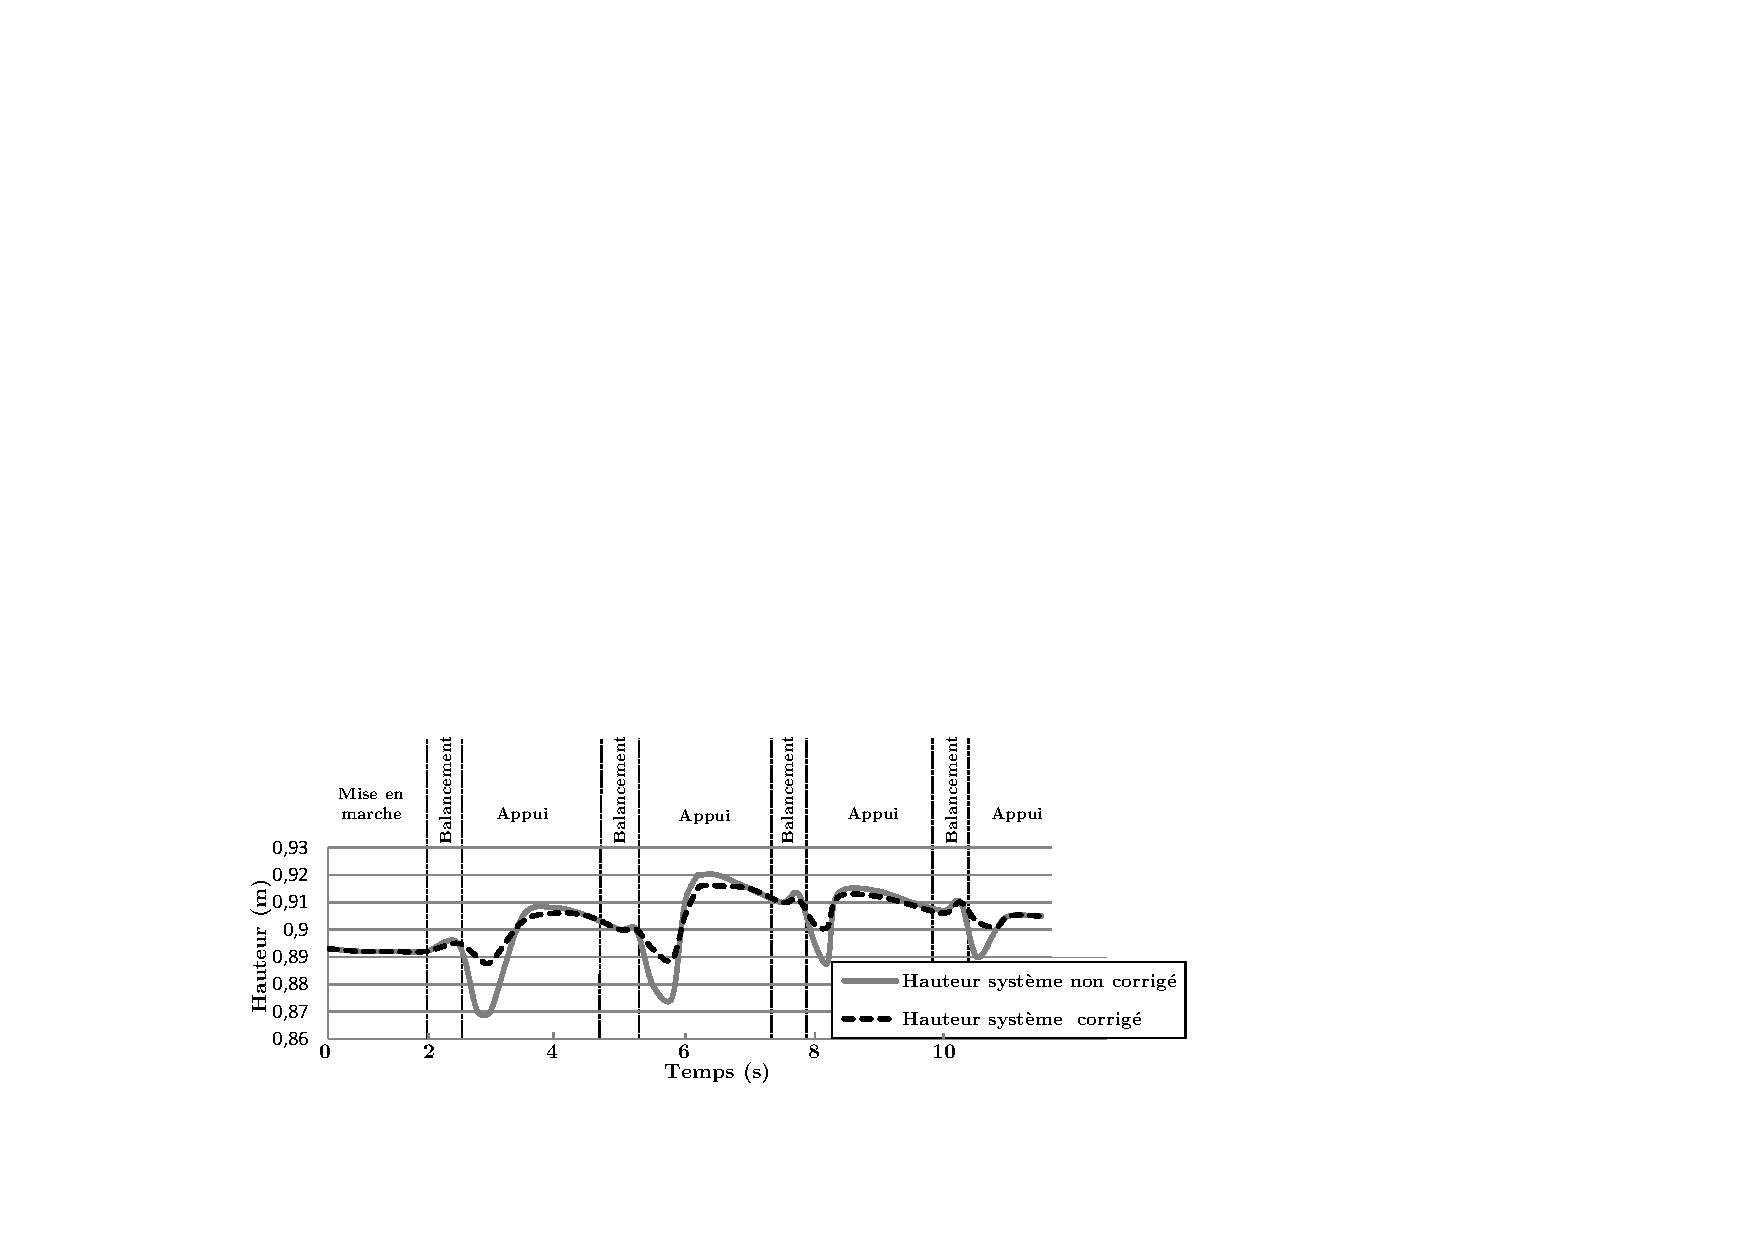
\includegraphics[width=0.9\linewidth]{evol_hauteur_main.pdf}
%\begin{minipage}[c]{.9\linewidth}
   \captionof{figure}{
   { Hauteur de la main au cours de la marche pour $V = 0,22$ m/s
%Trait gris continu système non corrigé, trait noir pointillé système avec correction PI généralisée.
}
\label{fig:evol_hauteur_main}
}
%\end{minipage}
%\end{minipage}
\end{center}

La \ref{fig:evol_hauteur_main} donne les évolutions de la hauteur de main mesurées lors d'une marche assistée avec le prototype de canne à la vitesse $V = 0,22$ m/s.\\ La courbe grise en trait continu correspond au cas où l'axe linéaire est sans correction ($C(p) = 1$).\\ La courbe noire en trait pointillé correspond au cas où l'axe linéaire est corrigé (correction PI généralisée avec paramètres optimisés). \\Il est à remarquer que lors de cet essai, le patient avait pour consigne de conserver sa main immobile lors du déplacement. Cette condition est difficilement vérifiable en pratique car le patient ne peut pas vraiment se concentrer sur la position de sa main pendant la marche.
\vspace{1em}
\fi

\question{Conclure sur l'influence de la correction de l'axe linéaire sur le respect de l'exigence de maintien de la hauteur de main.}

\ifprof
\begin{corrige}
Le cahier des charges (performance Id 7) impose un écart de hauteur de main de 3 cm pour un cycle de marche. Sans correction, l'écart peut atteindre jusqu'à 4,5 cm, avec correction l'écart est limité à 2,5 cm maxi ce qui vérifie le cdcf.\\
Avec correction les variations de hauteur de la main sont donc moins importantes au commencement de la phase d'appui. Ceci apporte un confort dans l'utilisation avec le sentiment d'avoir une canne plus rigide (moins d'affaissement) lors de l'appui.
\end{corrige}
\fi


\ifprof
\else
\vspace{1em}
Les figures \ref{fig:suivi_pied_orientation_normale} et \ref{fig:suivi_pied_orientation_rapide} donnent pour $V = 0,22$ m/s (allure normale), respectivement pour $V = 0,29$ m/s (allure rapide), le suivi du pied de la jambe gauche par la canne observé au niveau du sol et le suivi de l'orientation de la cuisse gauche (angle $\theta_g$) par la canne (angle~$\theta$).


\begin{center}%[ht!]
%\centering
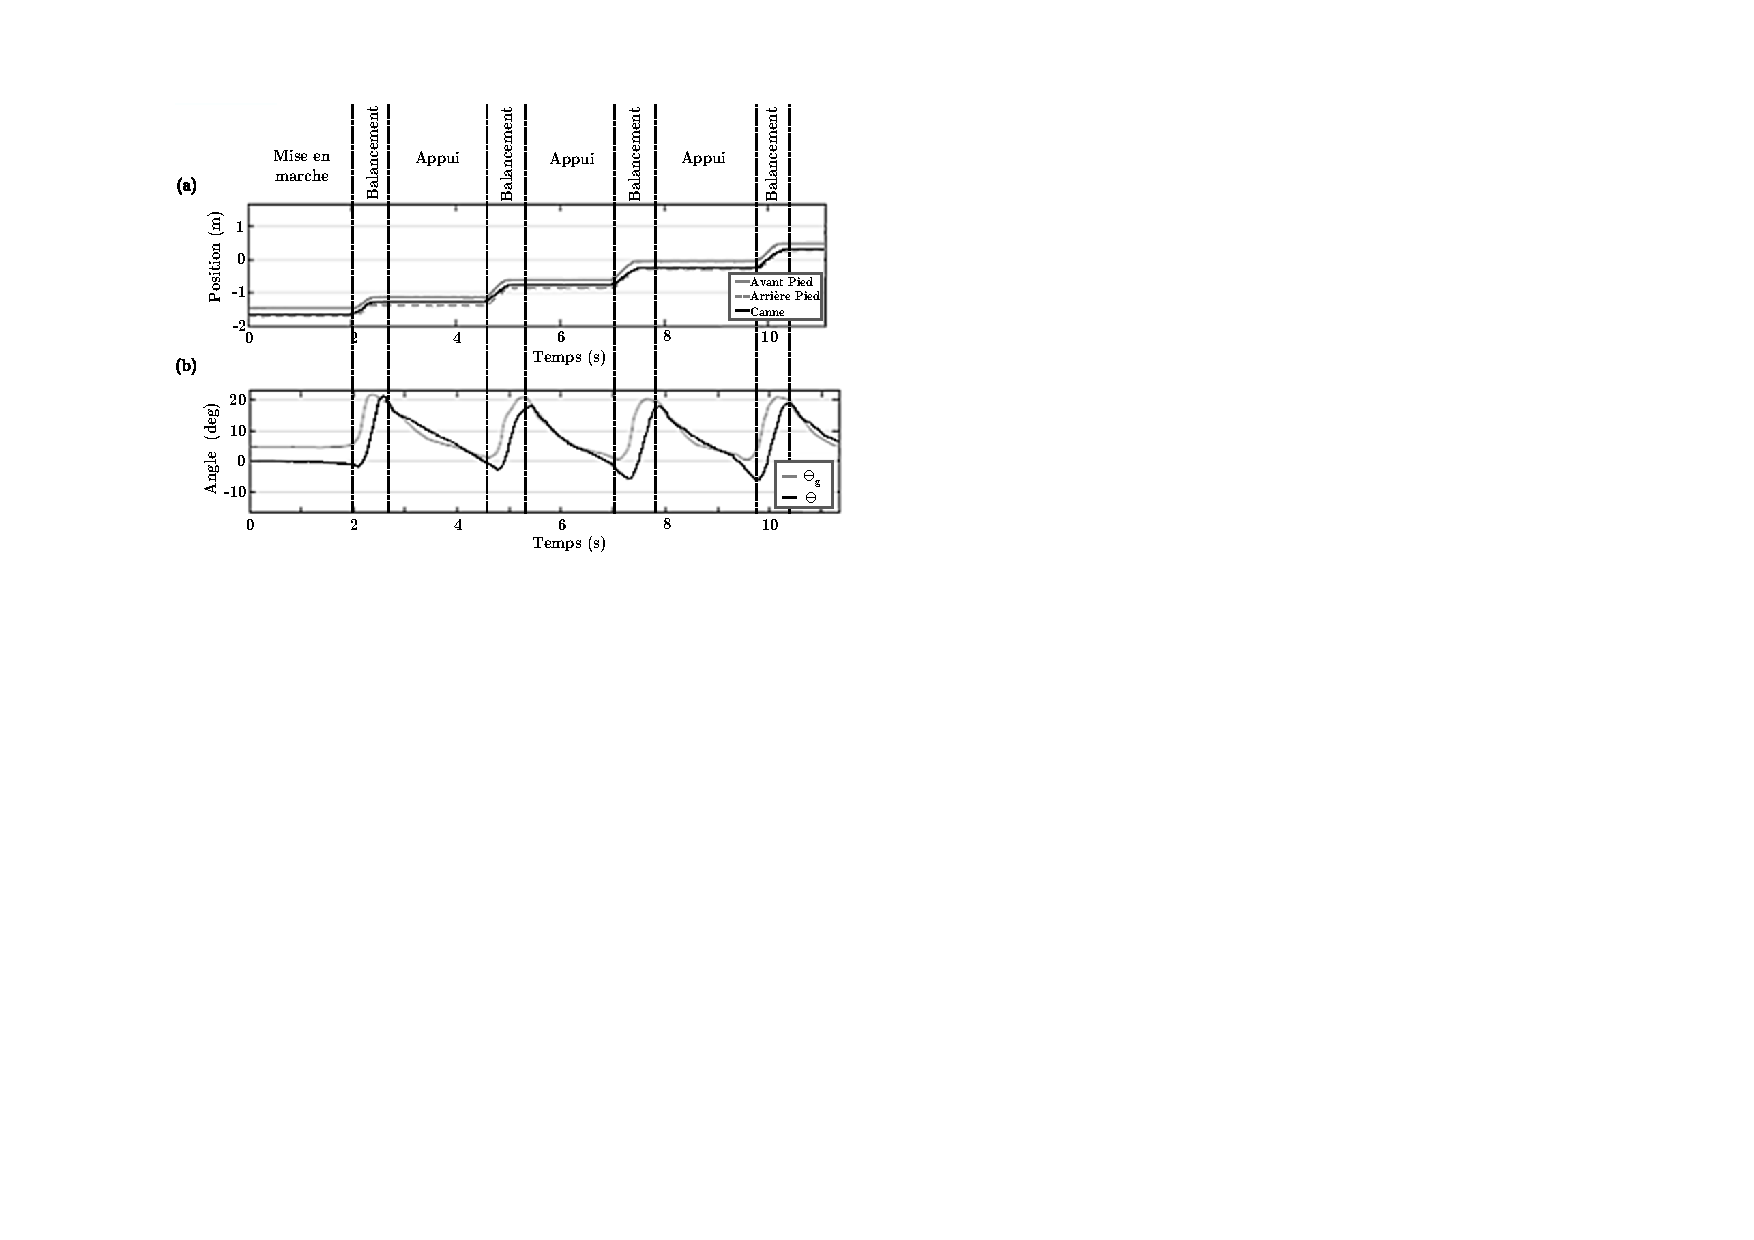
\includegraphics[width=0.9\linewidth]{suivi_pied_orientation_normale_.pdf}
   \captionof{figure}{{ $V = 0,22$ m/s, allure normale -- (a) : suivi du pied de la jambe gauche par la canne observé au niveau du sol -- (b) : suivi de l'orientation de la cuisse gauche (angle $\theta_g$) par la canne (angle $\theta$)} 
\label{fig:suivi_pied_orientation_normale}}
\end{center}

\begin{center}%M[!ht]
%\centering
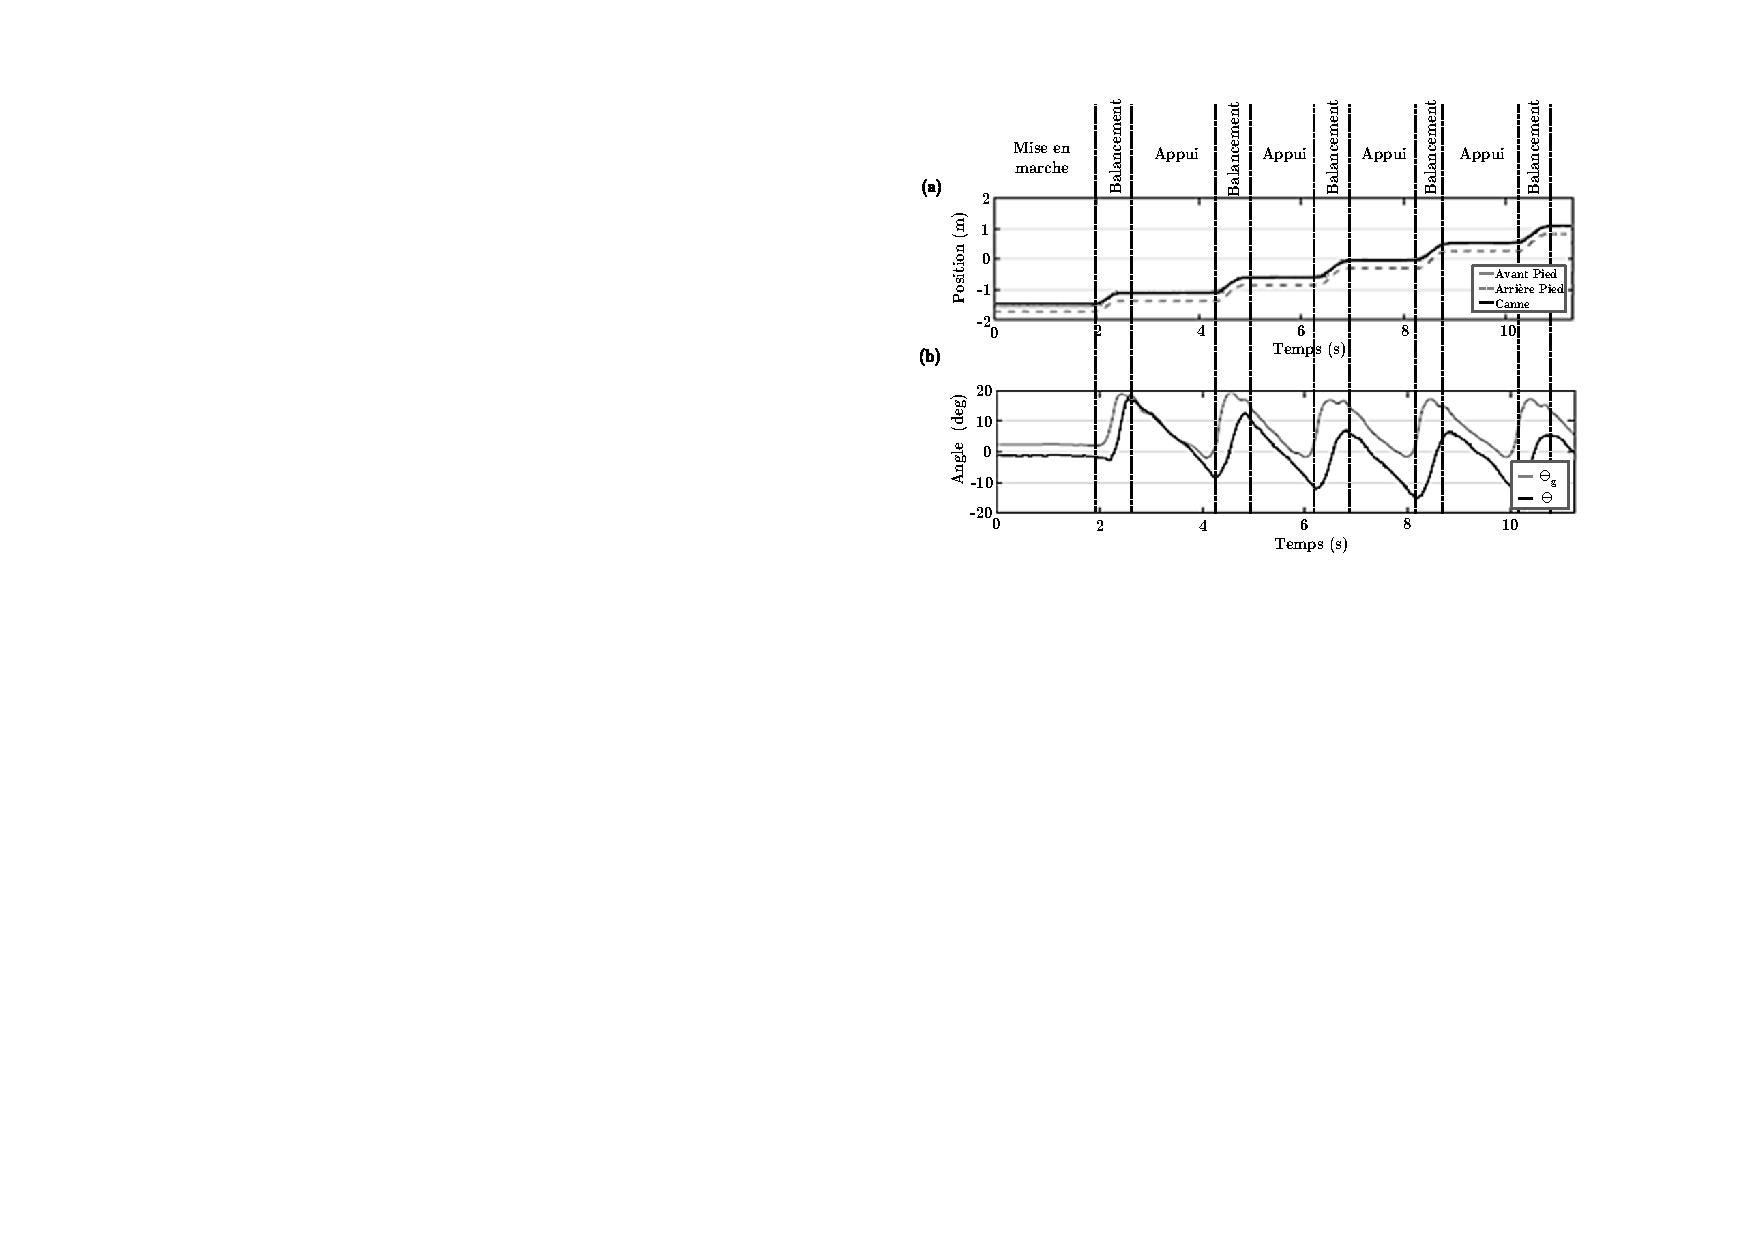
\includegraphics[width=0.9\linewidth]{suivi_pied_orientation_rapide_.pdf}
   \captionof{figure}{{ $V = 0,29$ m/s, allure rapide -- (a) : suivi du pied de la jambe gauche par la canne observé au niveau du sol -- (b) : suivi de l'orientation de la cuisse gauche (angle $\theta_g$) par la canne (angle $\theta$)}
\label{fig:suivi_pied_orientation_rapide}}
\end{center}

%\FloatBarrier

\fi

\question{Conclure sur le réglage des paramètres d'asservissement mis en place vis-à-vis des performances liées à la synchronisation de la canne avec le cycle locomoteur à différentes allures.}

\ifprof
\begin{corrige}
Le cahier des charges stipule comme performance à atteindre pour l'assistance de la marche (cadre Id 7) :\\
- un écart maximal sur l'angle d'orientation entre la canne et la jambe de 20\degre,\\
- le respect de l'exigence de suivi du pied, l'appui au sol de la canne doit se situer entre l'avant et l'arrière du pied de la jambe invalide.\\
Pour les deux allures de marche, l'exigence de suivi de pied est respectée car la courbe de position de la canne reste comprise entre les courbes de position de l'avant du pied et de l'arrière du pied (c'est à la limite de l'avant du pied pour le cas de la marche rapide).\\
Pour ce qui concerne l'exigence sur l'angle d'orientation, pour les deux allures l'exigence est respectée car les écarts restent inférieurs à 20\degre. Mise à part la phase d'appui en allure normale, l'orientation de la canne est en retard par rapport à l'orientation de la jambe, et ce retard est d'autant plus important que l'allure de la marche est élevée.\\
On peut donc conclure que ce réglage des paramètres d'asservissement permet de satisfaire les performances liées à la synchronisation de la canne avec le cycle locomoteur à différentes allures.
\end{corrige}
\fi




\ifprof
\else
\subsection*{Annexes -- Diagramme partiel des exigences\label{Annexe_diag_exigences}}
\begin{center}
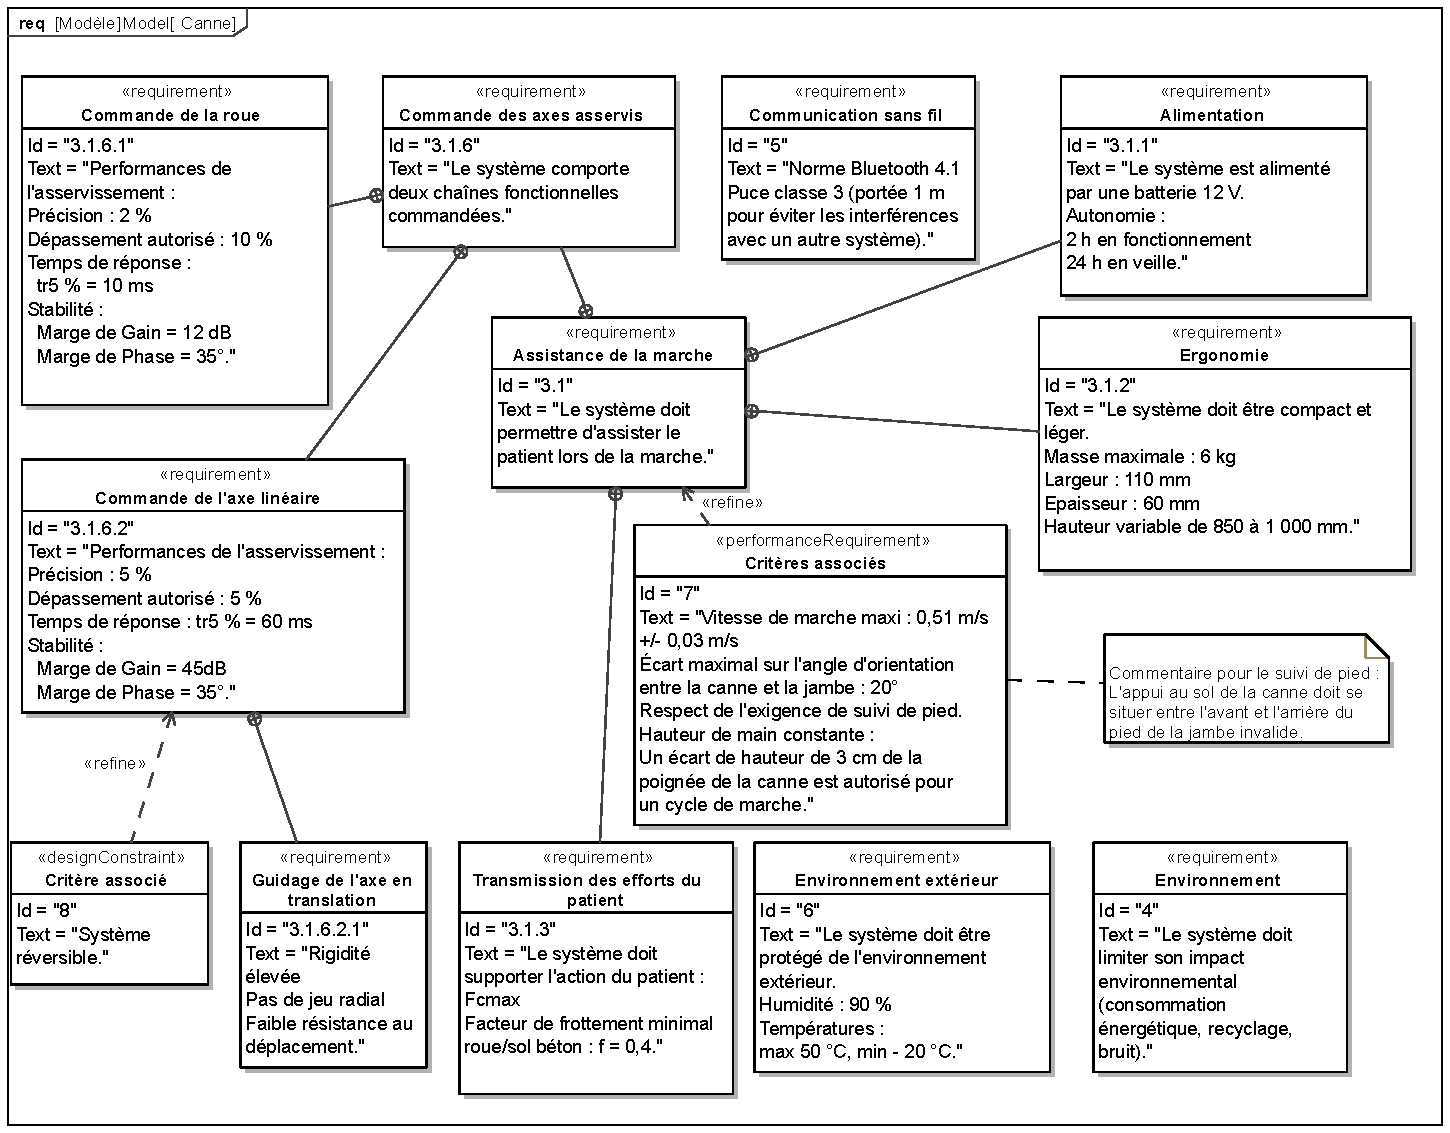
\includegraphics[width=\linewidth]{req_.pdf}

%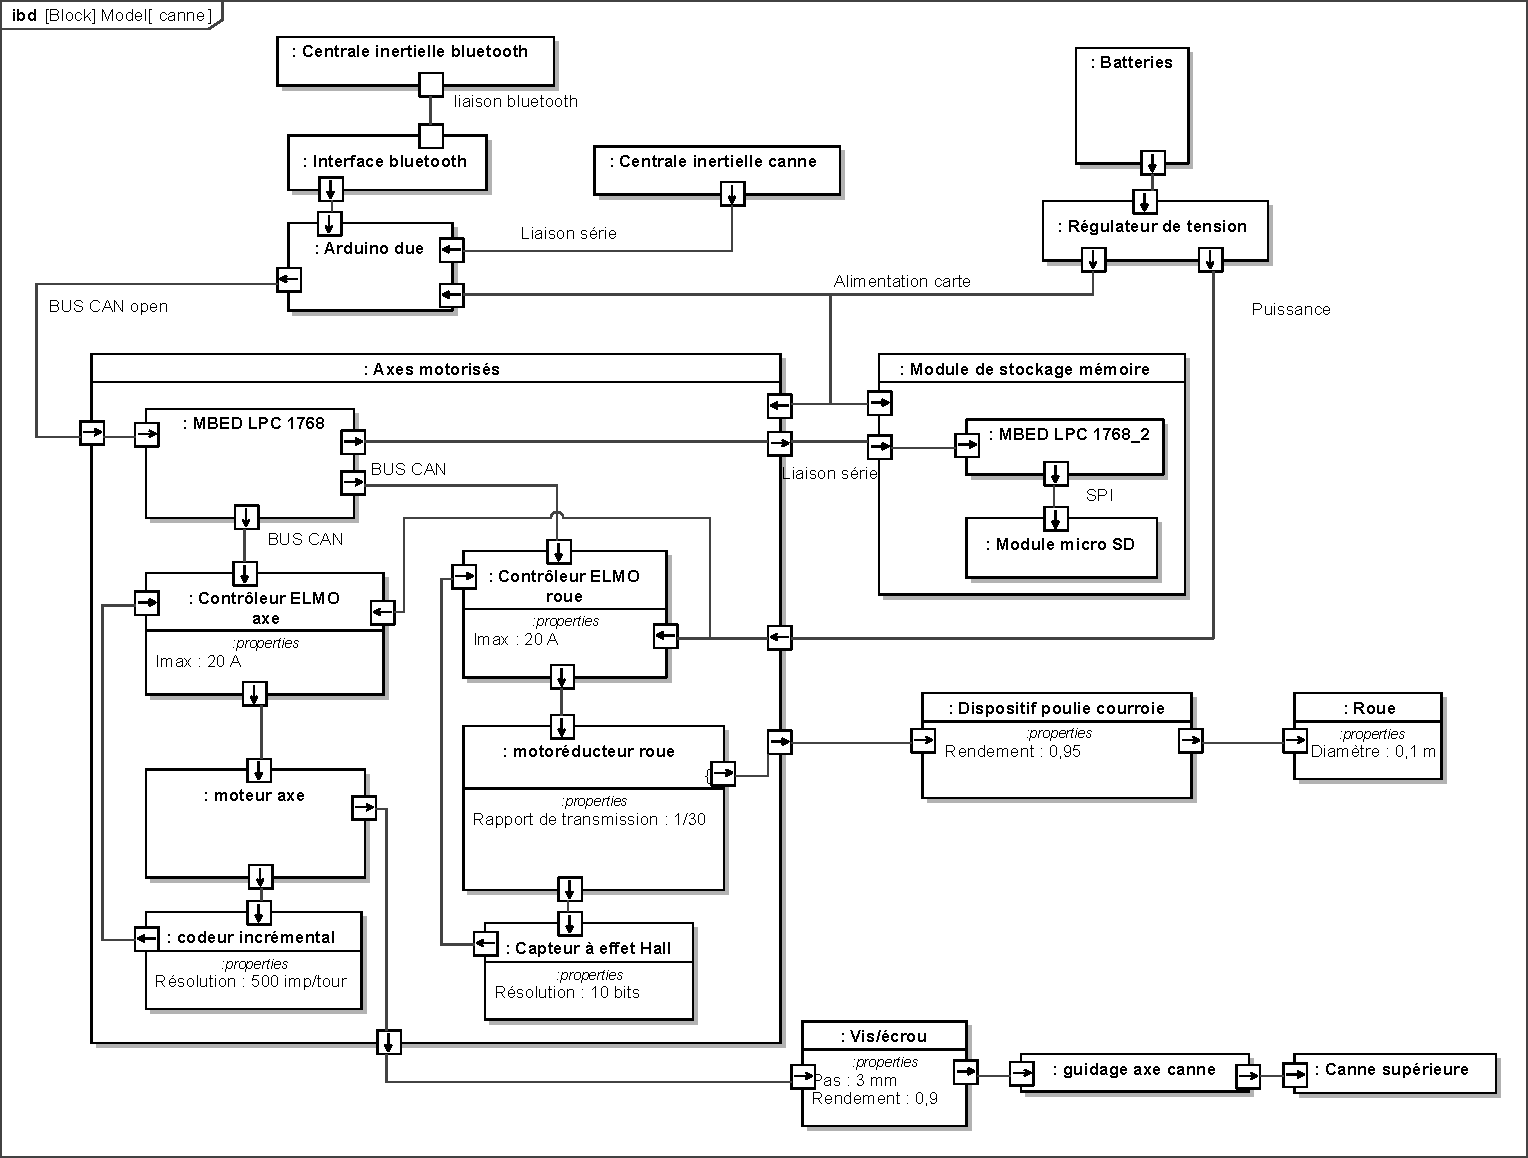
\includegraphics[width=\linewidth]{ibd.pdf}
\end{center}
%}
\fi





%%%%%%%%%%%%%%%%%%%%%%%%%%%%%%%%%%%%%%%%%%%%%%%%%%%

\ifprof
\else
\end{multicols}
\fi


\ifprof
\else


\begin{center}
%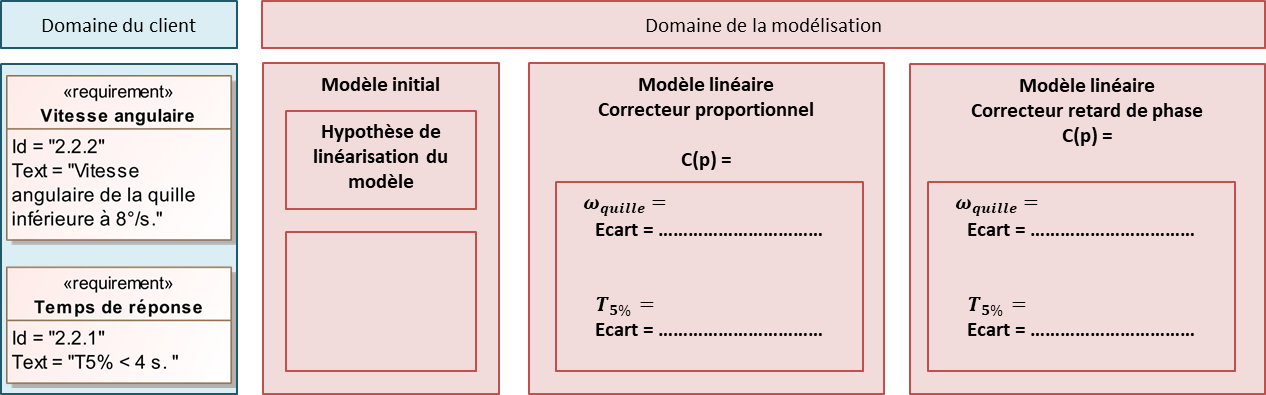
\includegraphics[width=\linewidth]{ecart}
%\textit{}
\end{center}

\begin{center}
%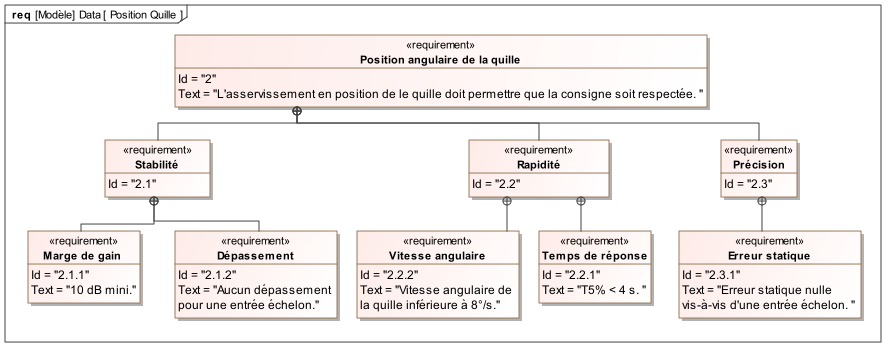
\includegraphics[width=.9\linewidth]{PositionQuille}
\end{center}


\fi
%
%\end{document}
%
%\question{}
%\ifprof
%\begin{corrige}
%\end{corrige}
%\else
%\fi
%
%\begin{center}
%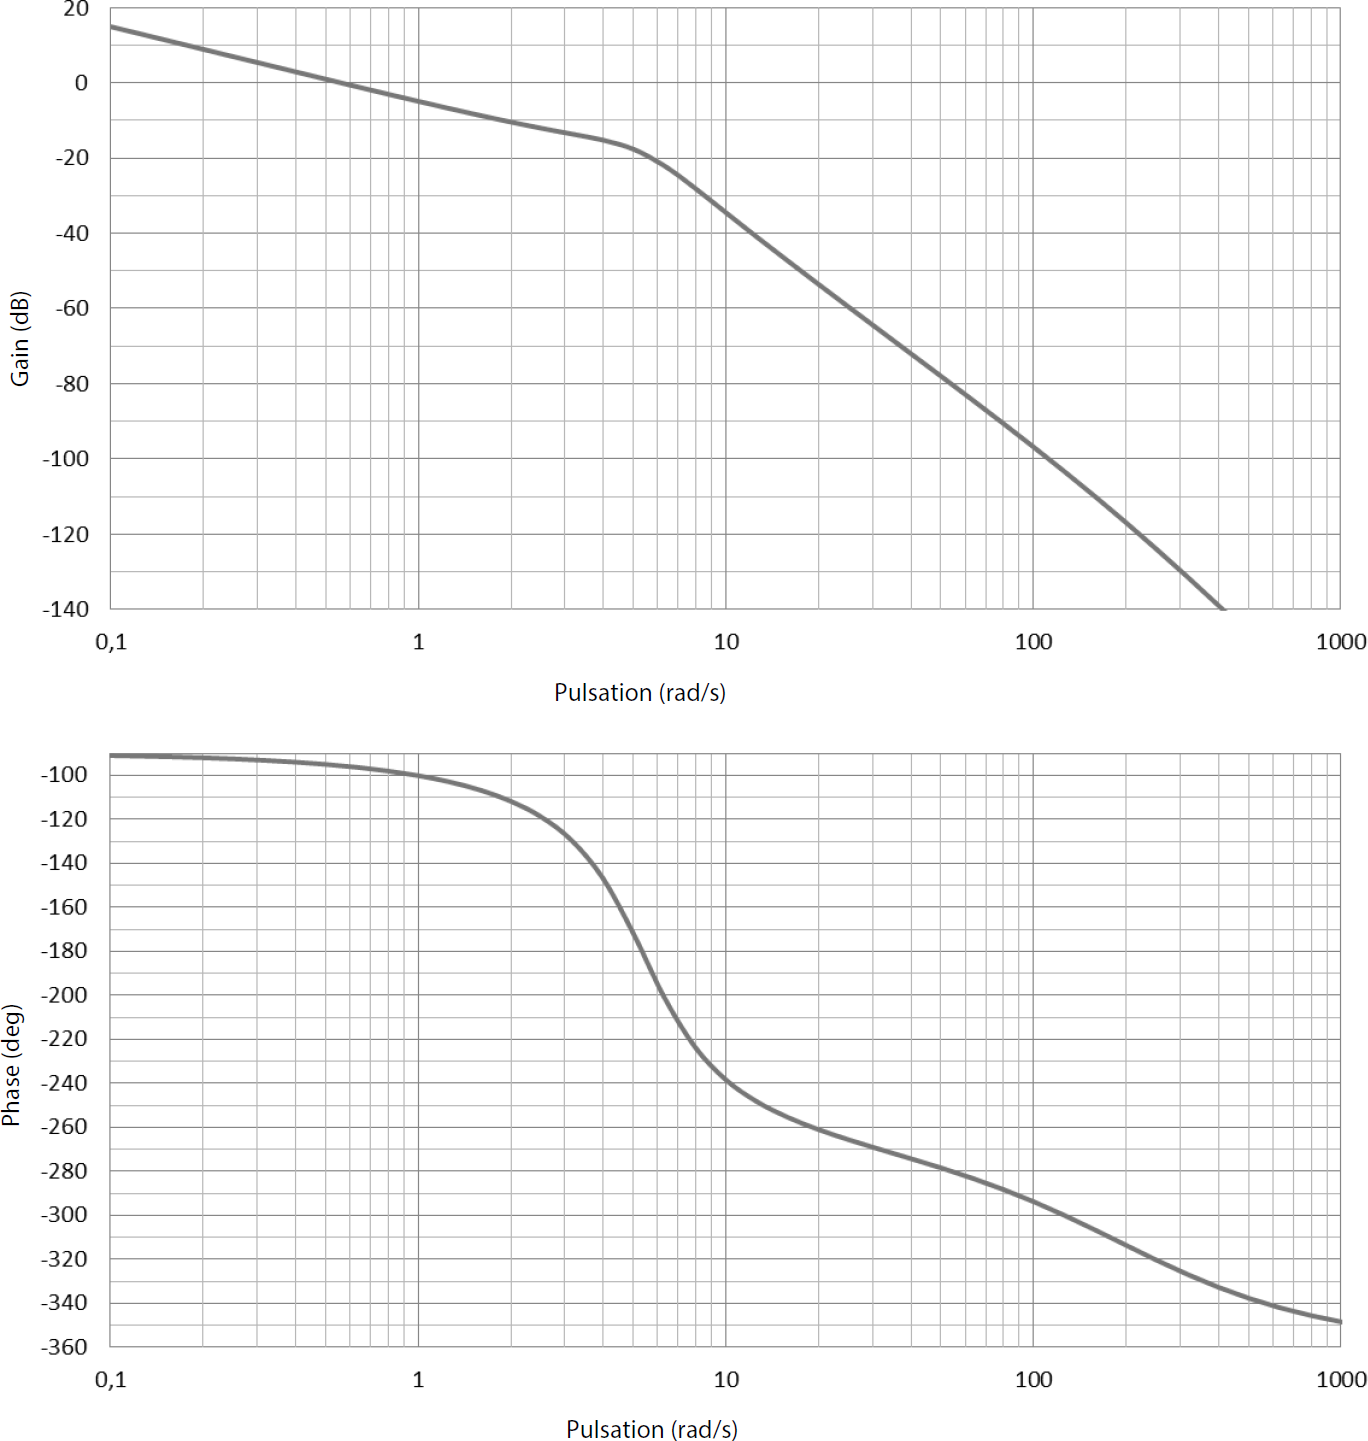
\includegraphics[width=\linewidth]{fig_04}
%%\textit{}
%\end{center}

